%{{{ Präämbel
%\documentclass[draft]{beamer} %% normal document
\documentclass[]{beamer} %% normal document
\usepackage{fontspec, unicode-math, caption, float, filecontents, verbatim}
\usepackage[ngerman]{babel}

%{{{ Beamer Stuff
\usetheme{Frankfurt}
\useoutertheme{default}
%\useoutertheme{split}
%\useinnertheme{rectangles}
\useinnertheme{circles}

%\setbeamertemplate{caption}[numbered]
%\captionsetup{labelformat=simple,font=scriptsize,labelfont=scriptsize}
\beamertemplatenavigationsymbolsempty

% puts Frame numbers in Dresden template
\newcommand*\oldmacro{}%
\let\oldmacro\insertshorttitle%
\renewcommand*\insertshorttitle{%
	\oldmacro\hfill%
	\insertframenumber\,/\,\inserttotalframenumber}

\logo{\pgfimage[width=2cm,height=2cm]{material/schlangenlogo}}
\newcommand{\nologo}{\setbeamertemplate{logo}{}} % command to set the logo to nothing

\title[]{Messtechnikpraktikum, Versuch 3}
\subtitle[]{Oszilloskope und ihre Tücken}
\date{\today}
%}}}

%{{{
\institute[Uni HD]{ Universität Heidelberg }
%}}}

%{{{
\author{ Moritz Nöltner }
%}}}


%{{{ Changemargin

\newenvironment{changemargin}[2]
{
	\begin{list}{}
		{
			\setlength{\topsep}{0pt}
			\setlength{\leftmargin}{#1}
			\setlength{\rightmargin}{#2}
			\setlength{\listparindent}{\parindent}
			\setlength{\itemindent}{\parindent}
			\setlength{\parsep}{\parskip}
		}
	\item[]
	}
	{
	\end{list}
}
%}}}

\AtBeginSection[]{
	\begin{frame}<beamer>
		\frametitle{Überblick}
		\tableofcontents[currentsection]
	\end{frame}
}

%}}}

%{{{
\begin{document}
	%{{{
	\begin{frame}[plain]
		\titlepage
		\note{ }
	\end{frame}
	%}}}


	\section{Signalerfassung und Artefakte}
	%{{{
	\begin{frame}{Sinusschwingung}
		Oszi direkt mit Signalgenerator verbunden, 1kHz, Sinus\\

		\begin{tabular}{|l|l|}
			\hline
			Zeitbasis &  Schwingungen \\
			\hline
			\hline
			0,1 ms = 100 \mu s & 1\\
			\hline
			0,25 ms = 250 \mu s & 2.5\\
			\hline
			0,5 ms = 50 \mu s & 5\\
			\hline
			1 ms & 10 \\
			\hline
		\end{tabular}
	\end{frame}

	\begin{frame}
		\begin{figure}[H]
			\centering
			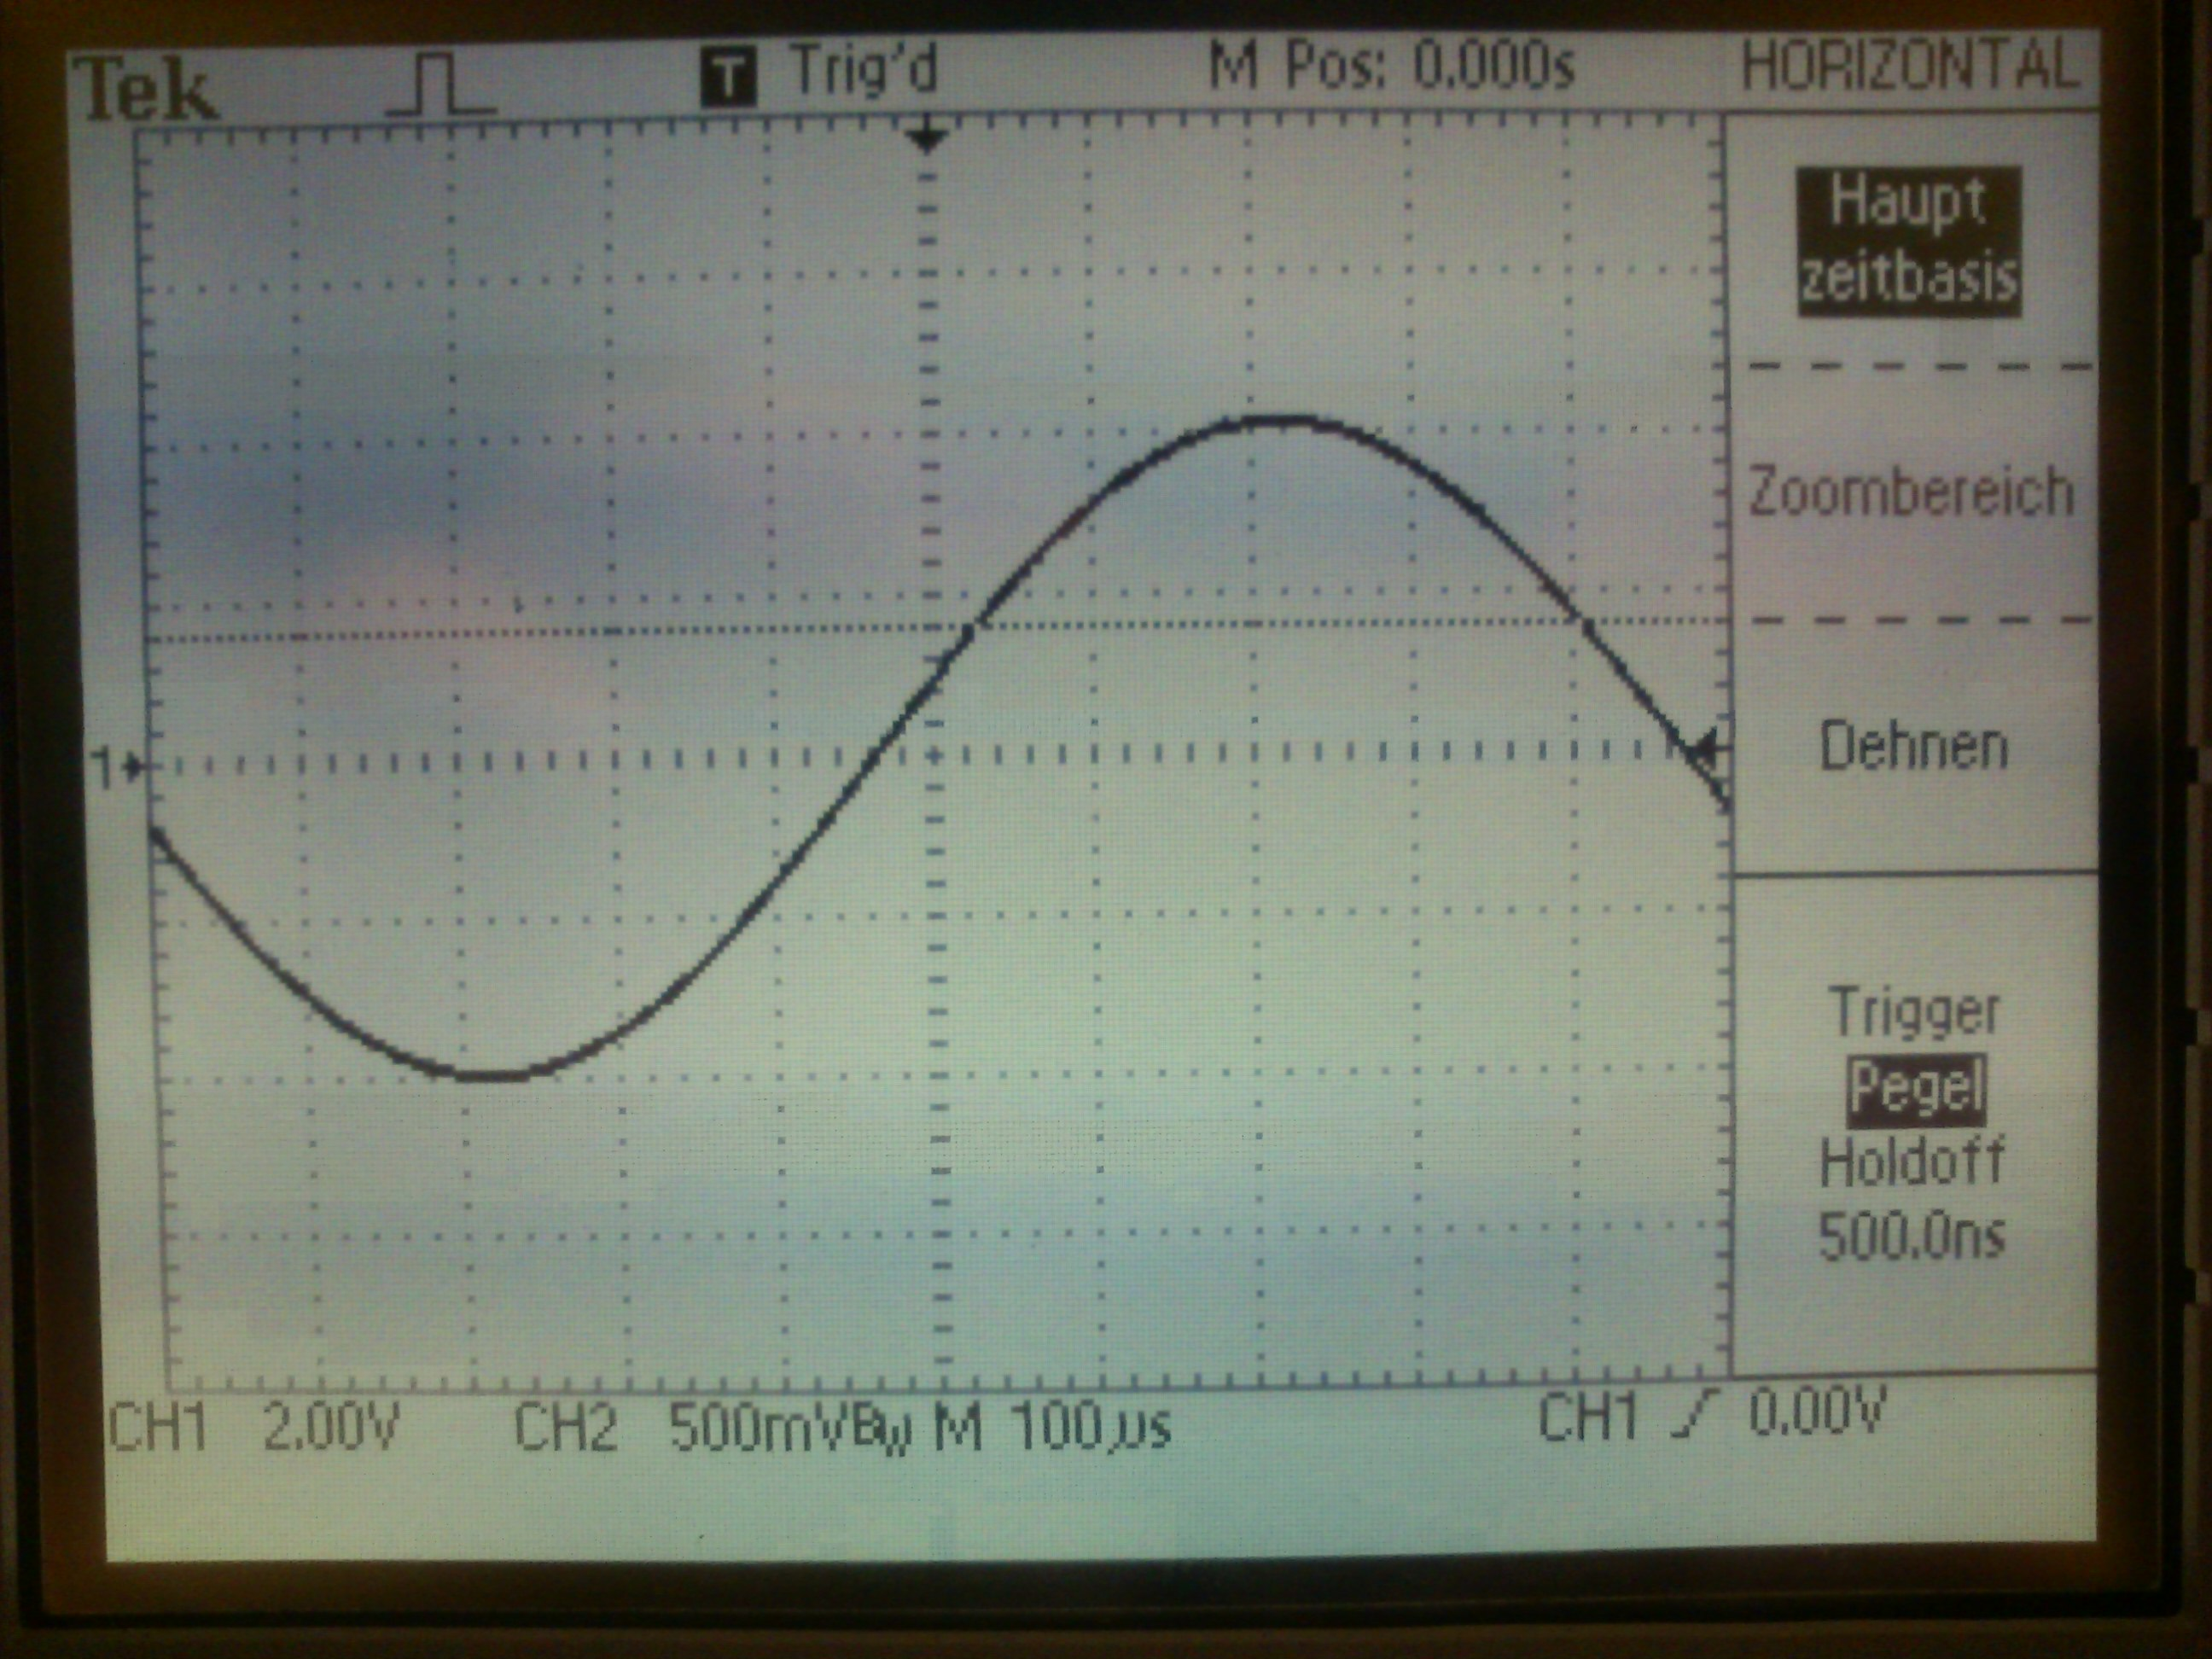
\includegraphics[width=0.8\linewidth]{../versuch3/oszibilder/DSC_0240.JPG}
			\caption{Sinusspannung durch Verstellen von Triggerlevel und Verzögerung mittig zentriert}
		\end{figure}
	\end{frame}


	\begin{frame}
		\begin{figure}[H]
			\centering
			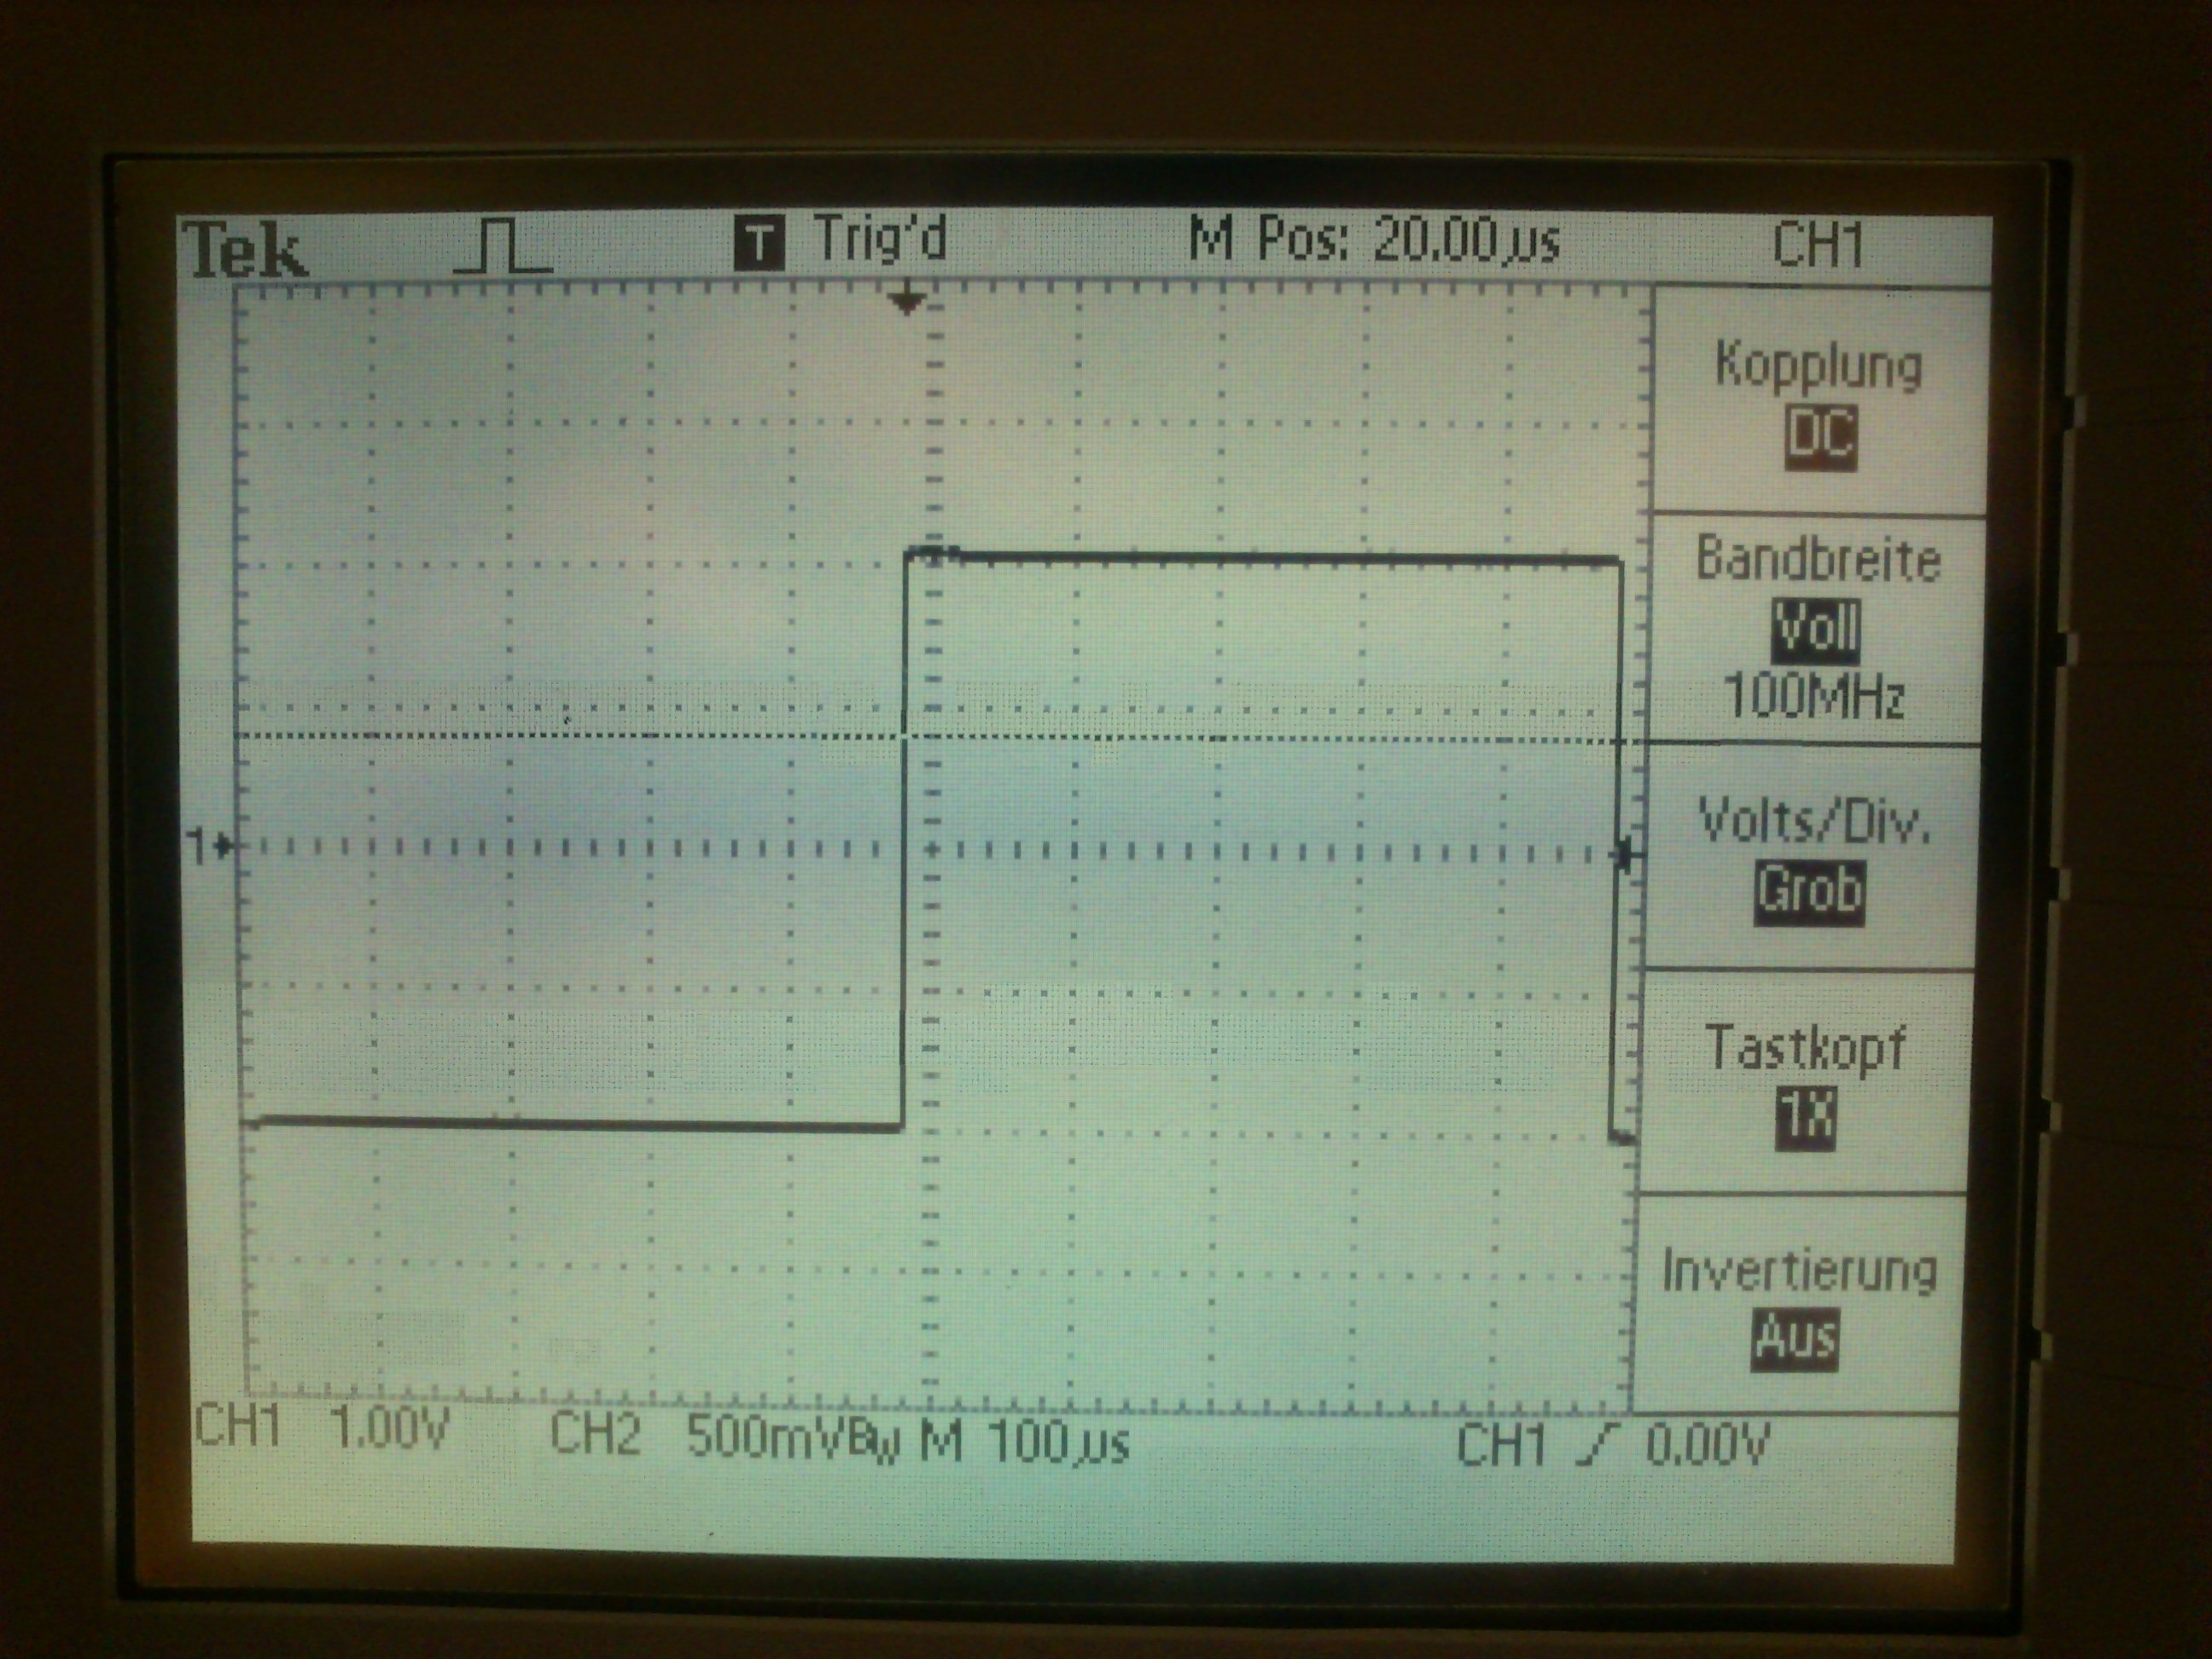
\includegraphics[width=.8\linewidth]{../versuch3/oszibilder/DSC_0246.JPG}
			\caption{Eine Rechteckspannung}
		\end{figure}
	\end{frame}


	\begin{frame}
		\begin{figure}[H]
			\centering
			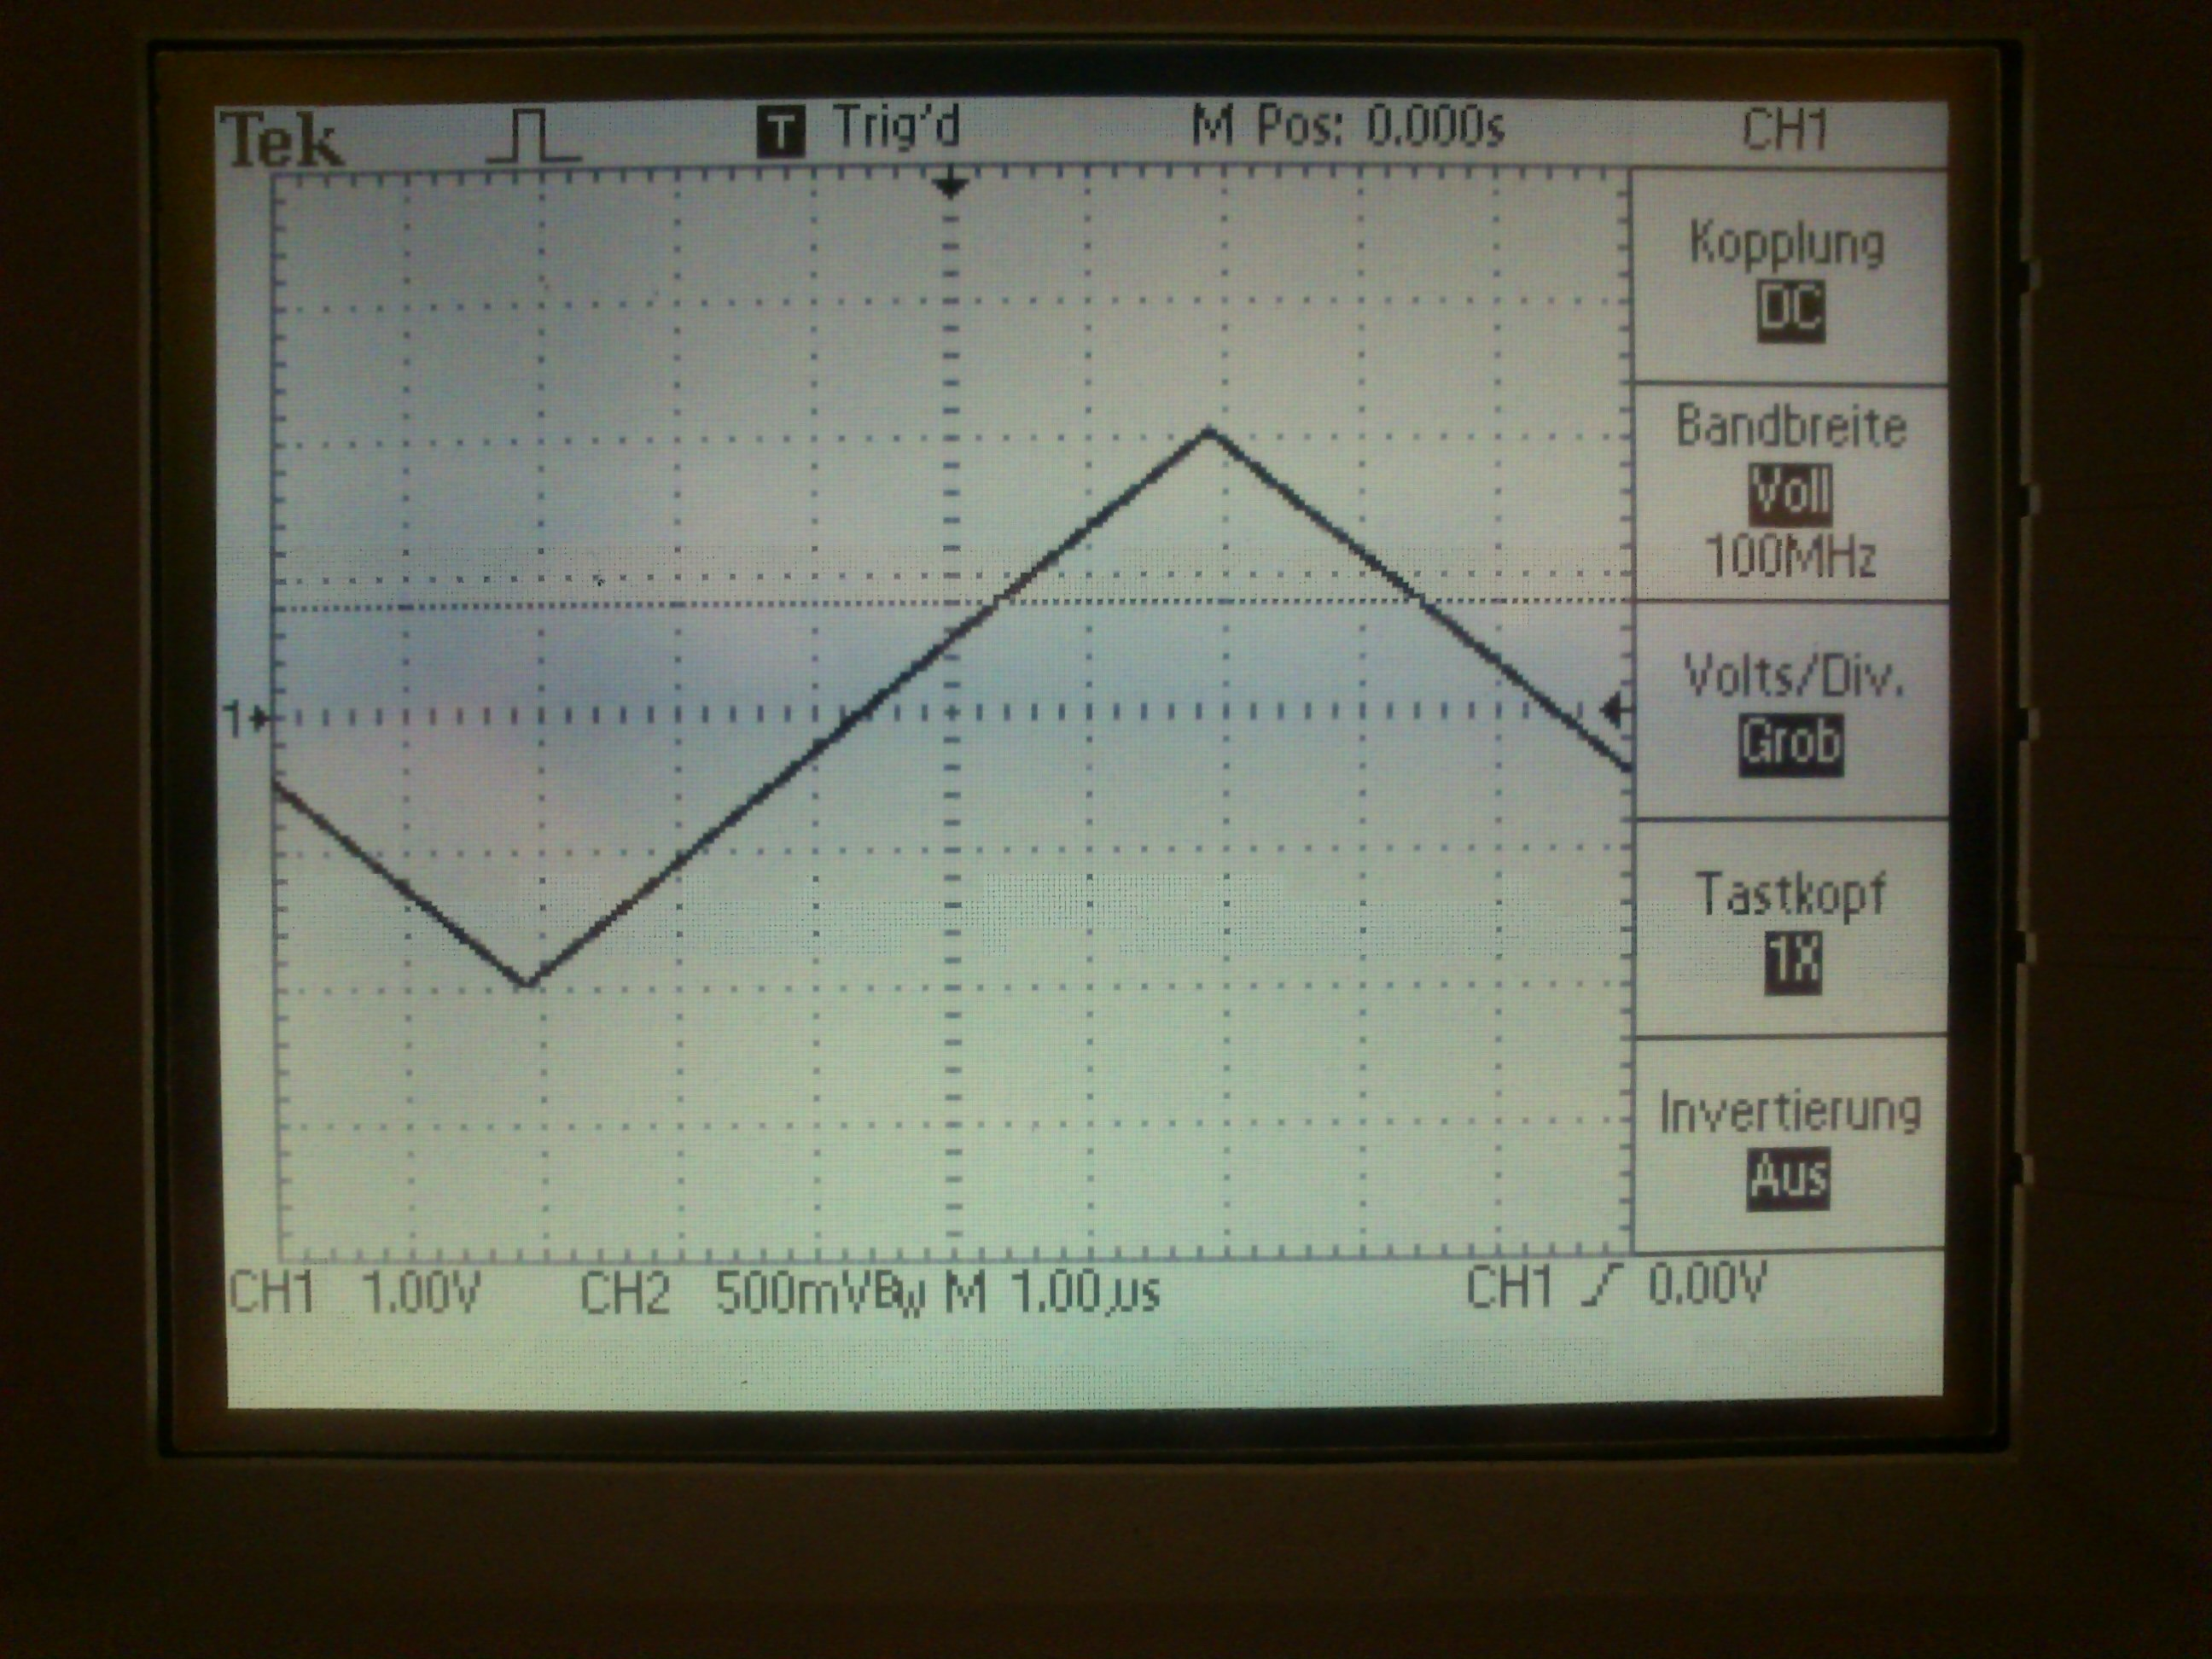
\includegraphics[width=.8\linewidth]{../versuch3/oszibilder/DSC_0252.JPG}
			\caption{Und eine Dreieckspannung}
		\end{figure}
	\end{frame}


	\begin{frame}
		Als nächstes wurde der Generator auf 1 MHz Sinus gestellt und mit dem Oszilloskop bei einer Zeitbasis von 1 µS die Frequenz gemessen:
		\begin{figure}[H]
			\centering
			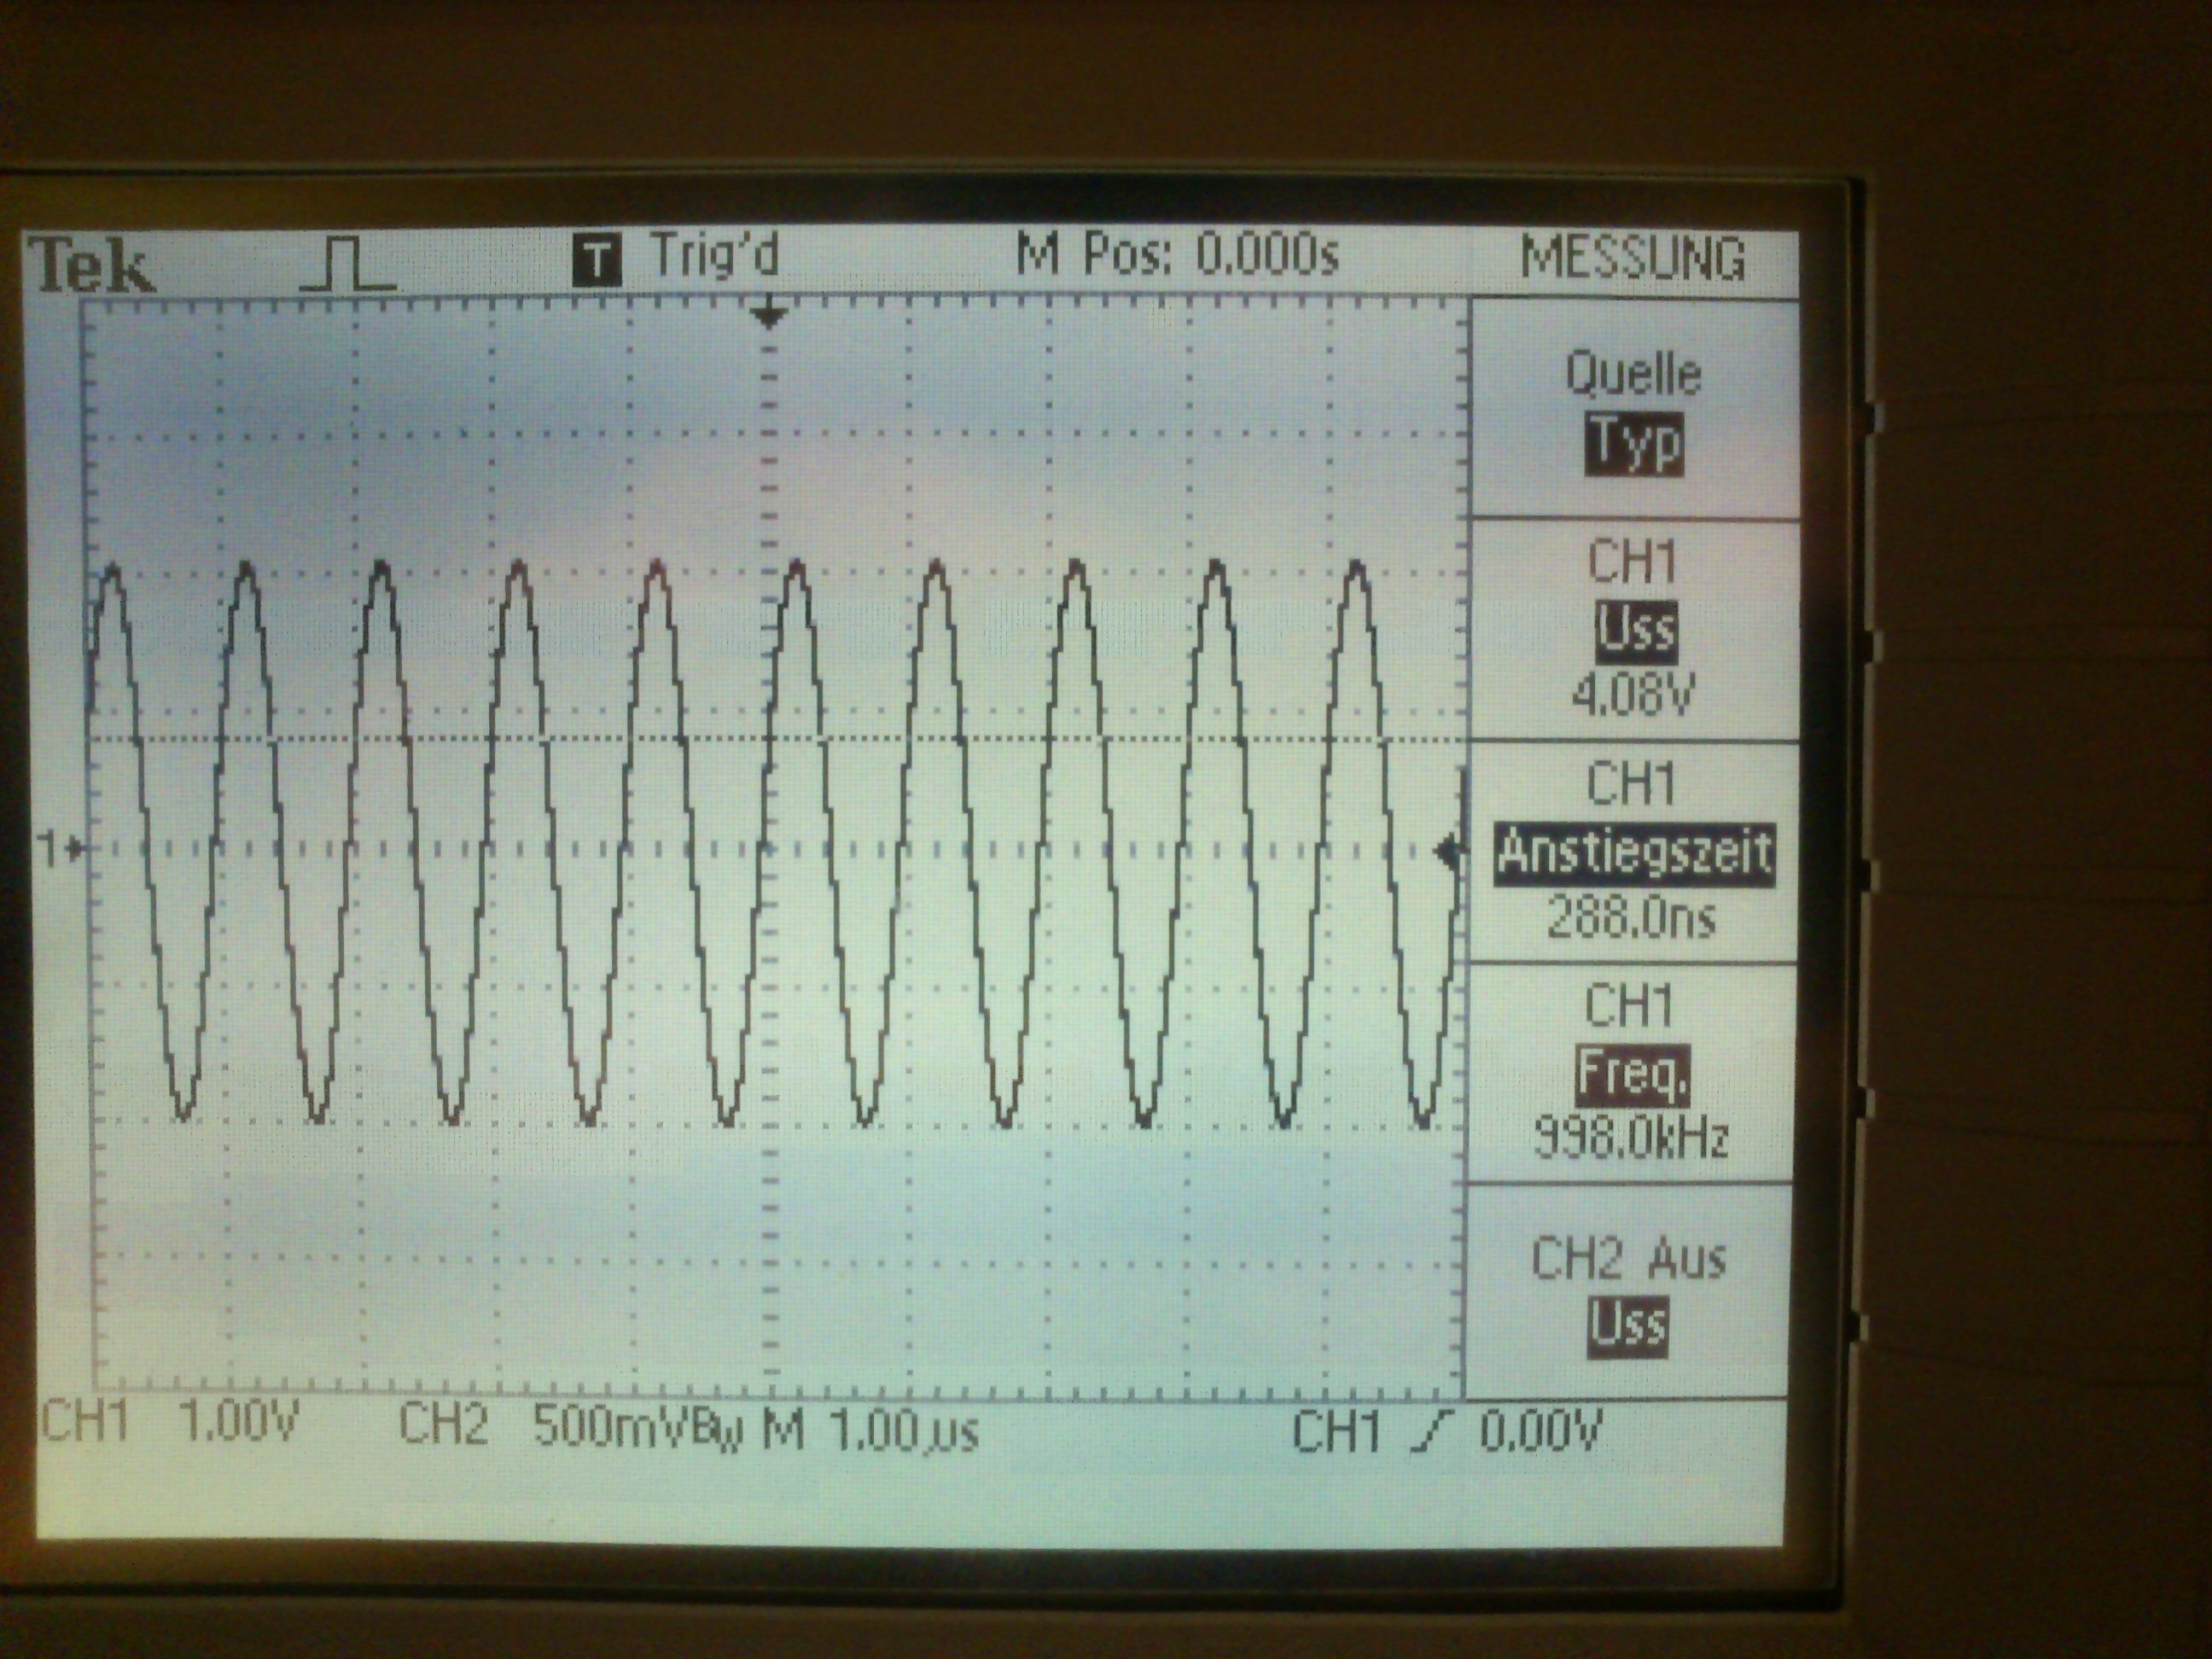
\includegraphics[width=.8\linewidth]{../versuch3/oszibilder/DSC_0253.JPG}
			\caption{Frequenzmessung bei 1 MHz und 1µs Zeitbasis}
		\end{figure}
	\end{frame}



	\section{Oszillators mit NE555}
	\begin{frame}{Berechnung der Frequenz}
		Zuerst sollte die Frequenz des Oszillators bestimmt werden:\\
		$ f=\frac{1}{T},\; T = 0,693 * (R_A + 2 R_B) * C;\; Ra = 1kΩ,\; Rb = 1kΩ,\; C = 4.7nF$\\
		$\Rightarrow f=\frac{1}{0,693 * (1kΩ + 2*1kΩ) * 4.7nF} = 102.35 kHz$\\
	\end{frame}

	\begin{frame}
		\begin{figure}[H]
			\centering
			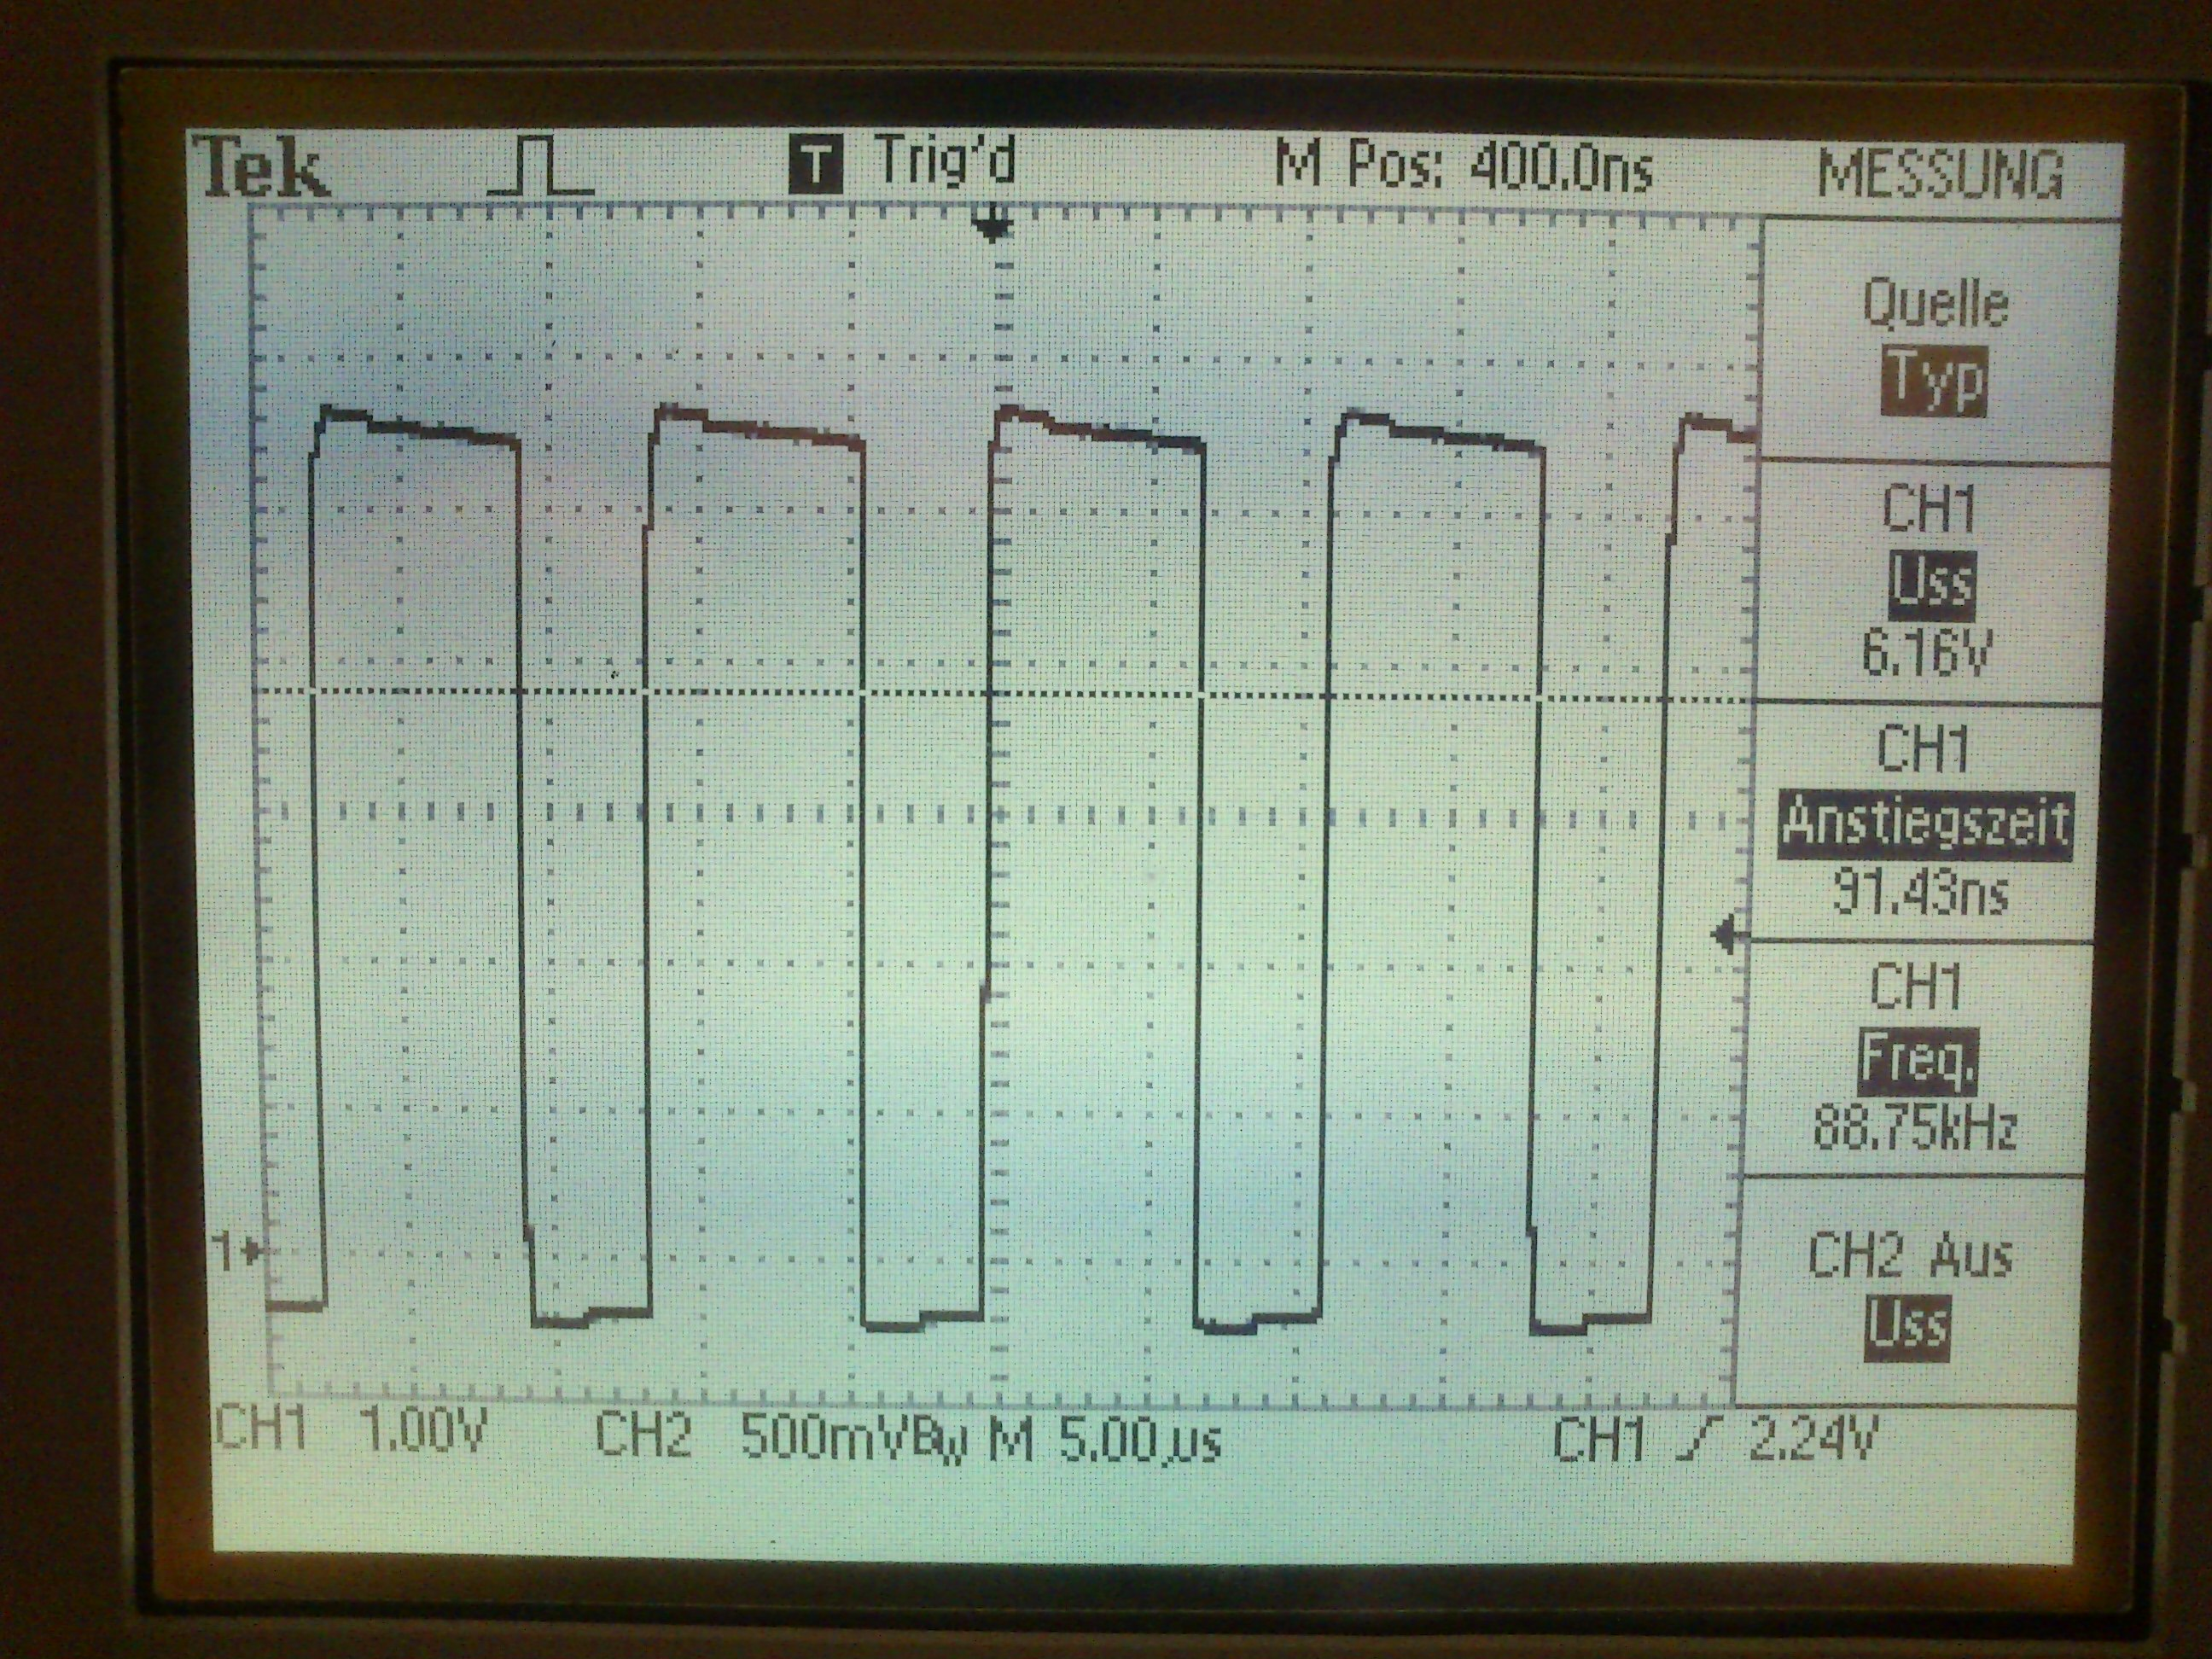
\includegraphics[width=.8\linewidth]{../versuch3/oszibilder/DSC_0259.JPG}
			\caption{Frequenzmessung der Oszillatorfrequenz}
		\end{figure}
	\end{frame}

	\begin{frame}
		\begin{figure}[H]
			\centering
			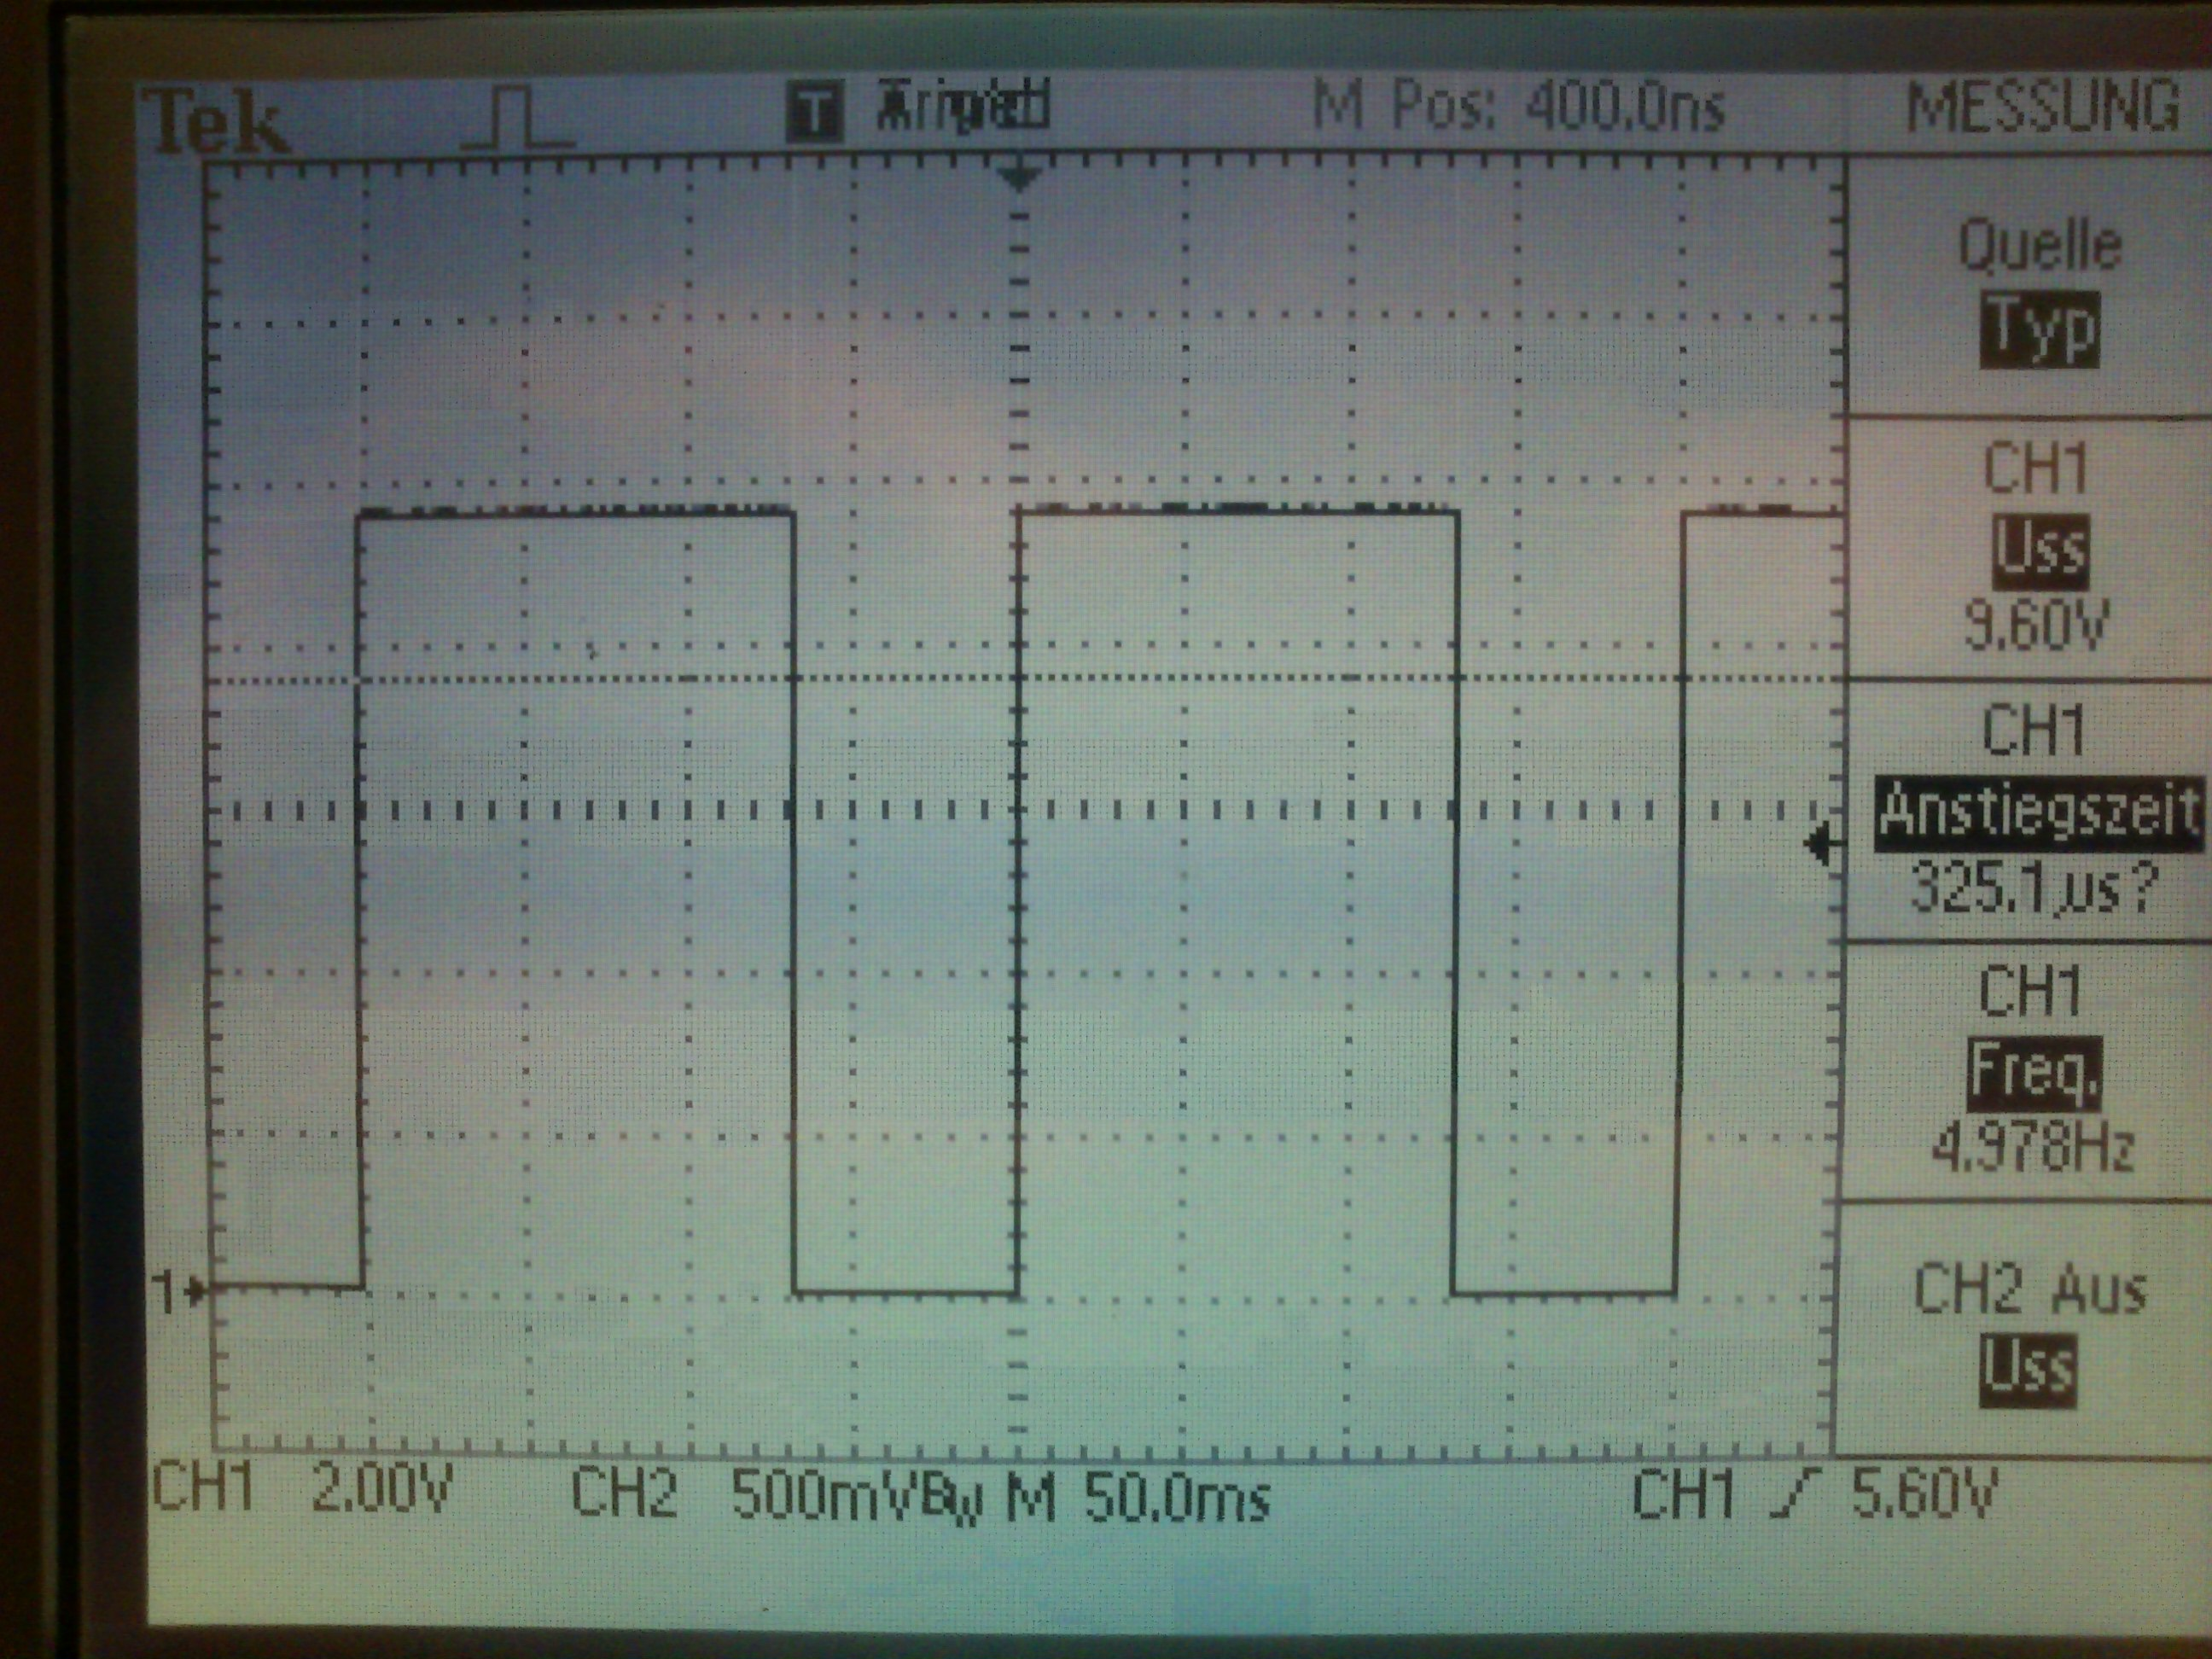
\includegraphics[width=.8\linewidth]{../versuch3/oszibilder/DSC_0268.JPG}
			\caption{Frequenzmessung bei vergrößerter Kapazität}
		\end{figure}
	\end{frame}

	\section{Hoch und Tiefpass}

	\begin{frame}
		\begin{figure}
			\centering
			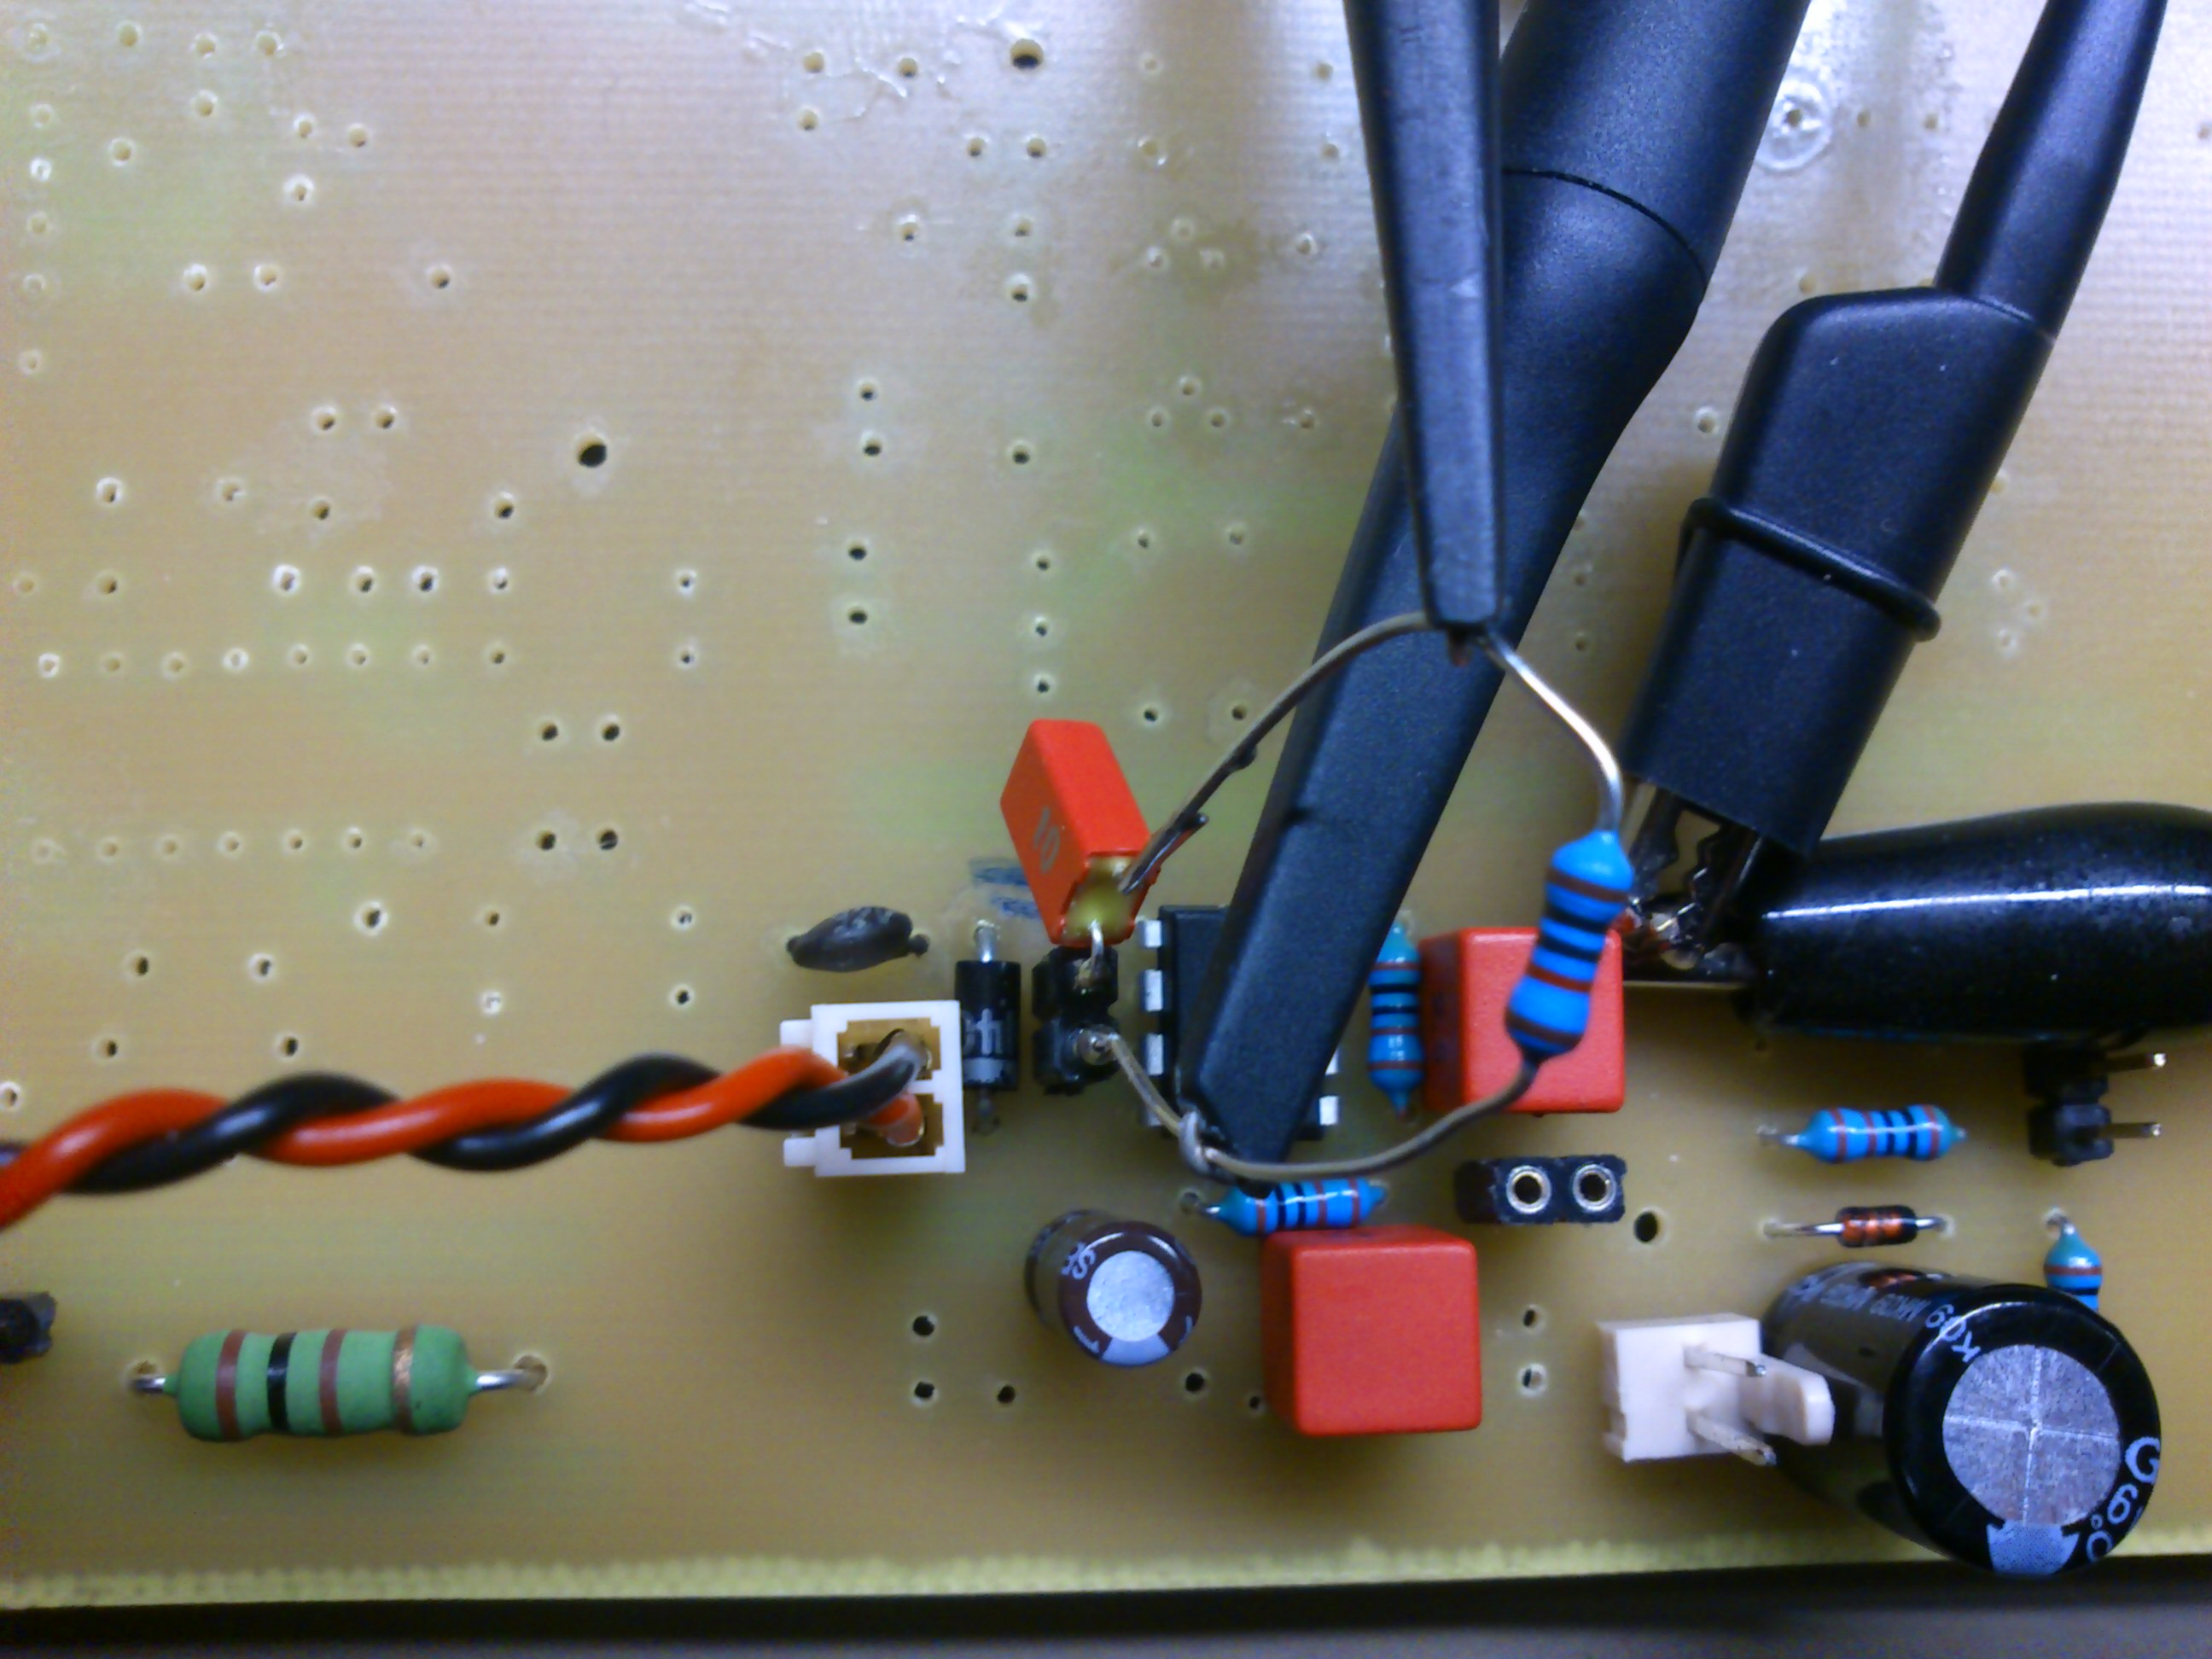
\includegraphics[width=.8\linewidth]{../versuch3/oszibilder/DSC_0274.JPG}
			\caption{Das eingebaute Filter}
		\end{figure}
	\end{frame}

	\begin{frame}
		Die Impulsantwort ergab sich wie folgt:
		\begin{figure}[H]
			\centering
			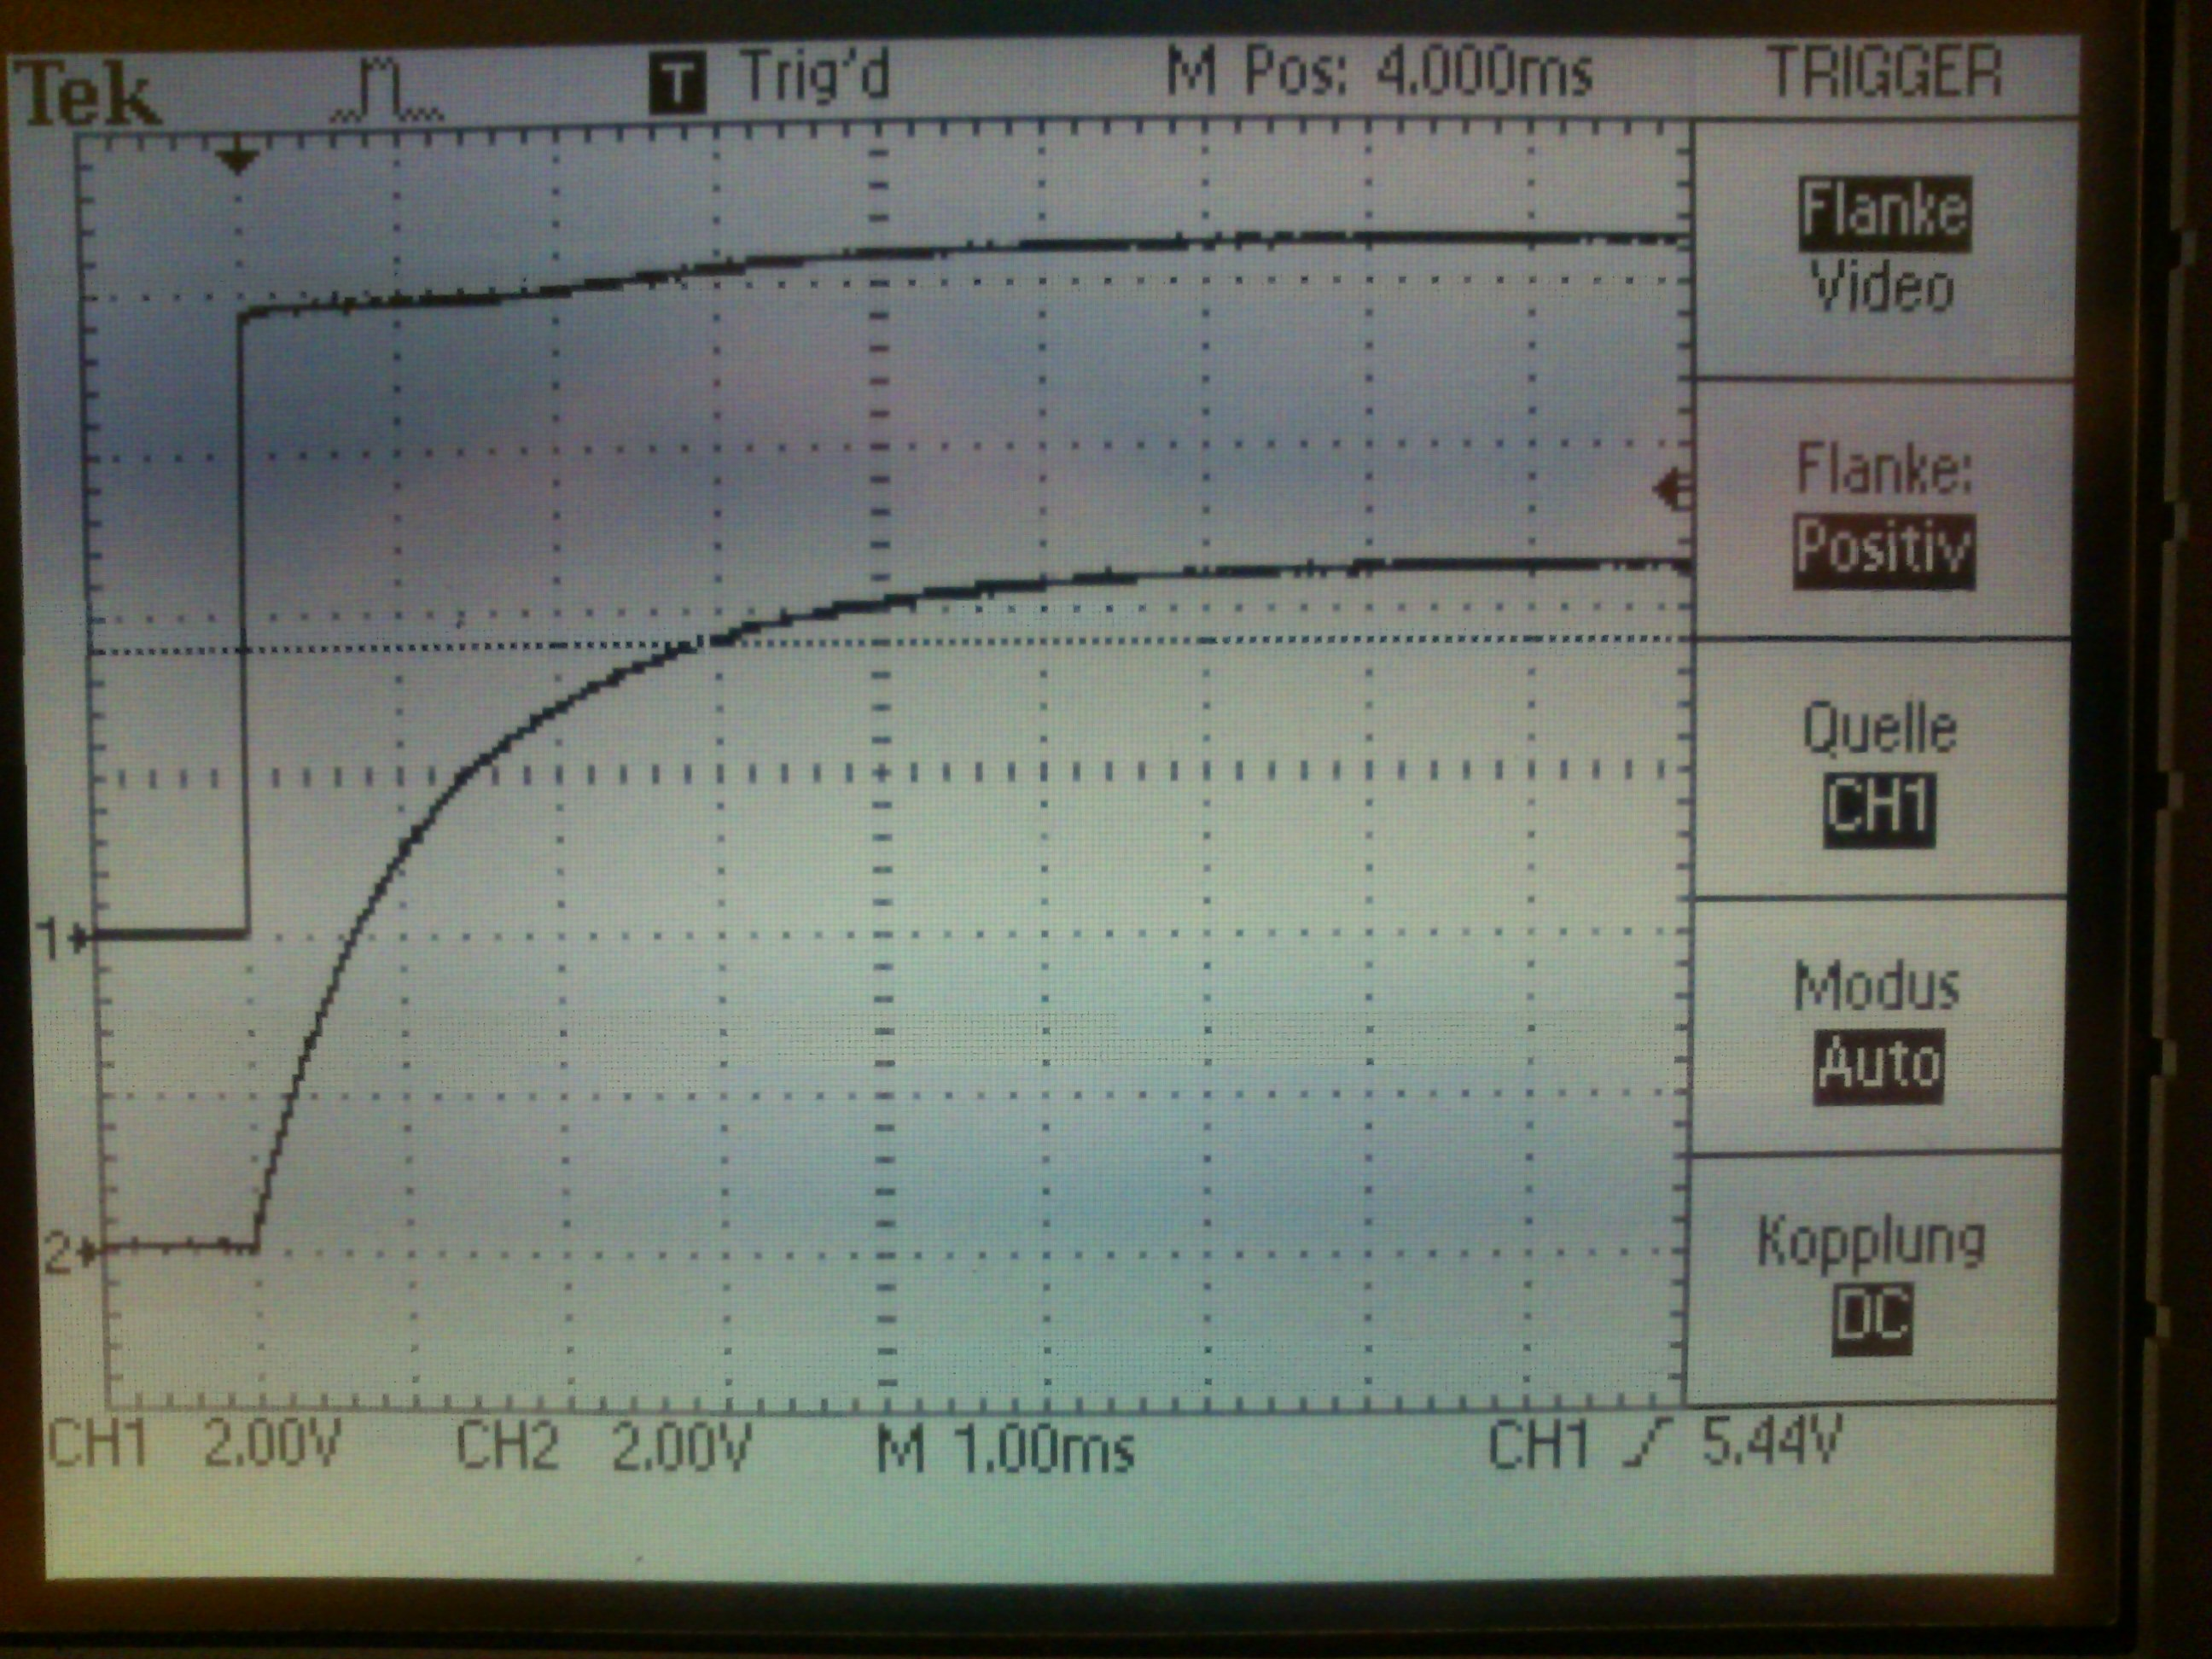
\includegraphics[width=.8\linewidth]{../versuch3/oszibilder/DSC_0283.JPG}
			\caption{Impulsantwort des Tiefpasses}
		\end{figure}
	\end{frame}

	\begin{frame}
		Dann wurde das Filter umgekehrt aufgesteckt, damit als Hochpass verwendet und dessen Impulsantwort bestimmt:
		\begin{figure}[H]
			\centering
			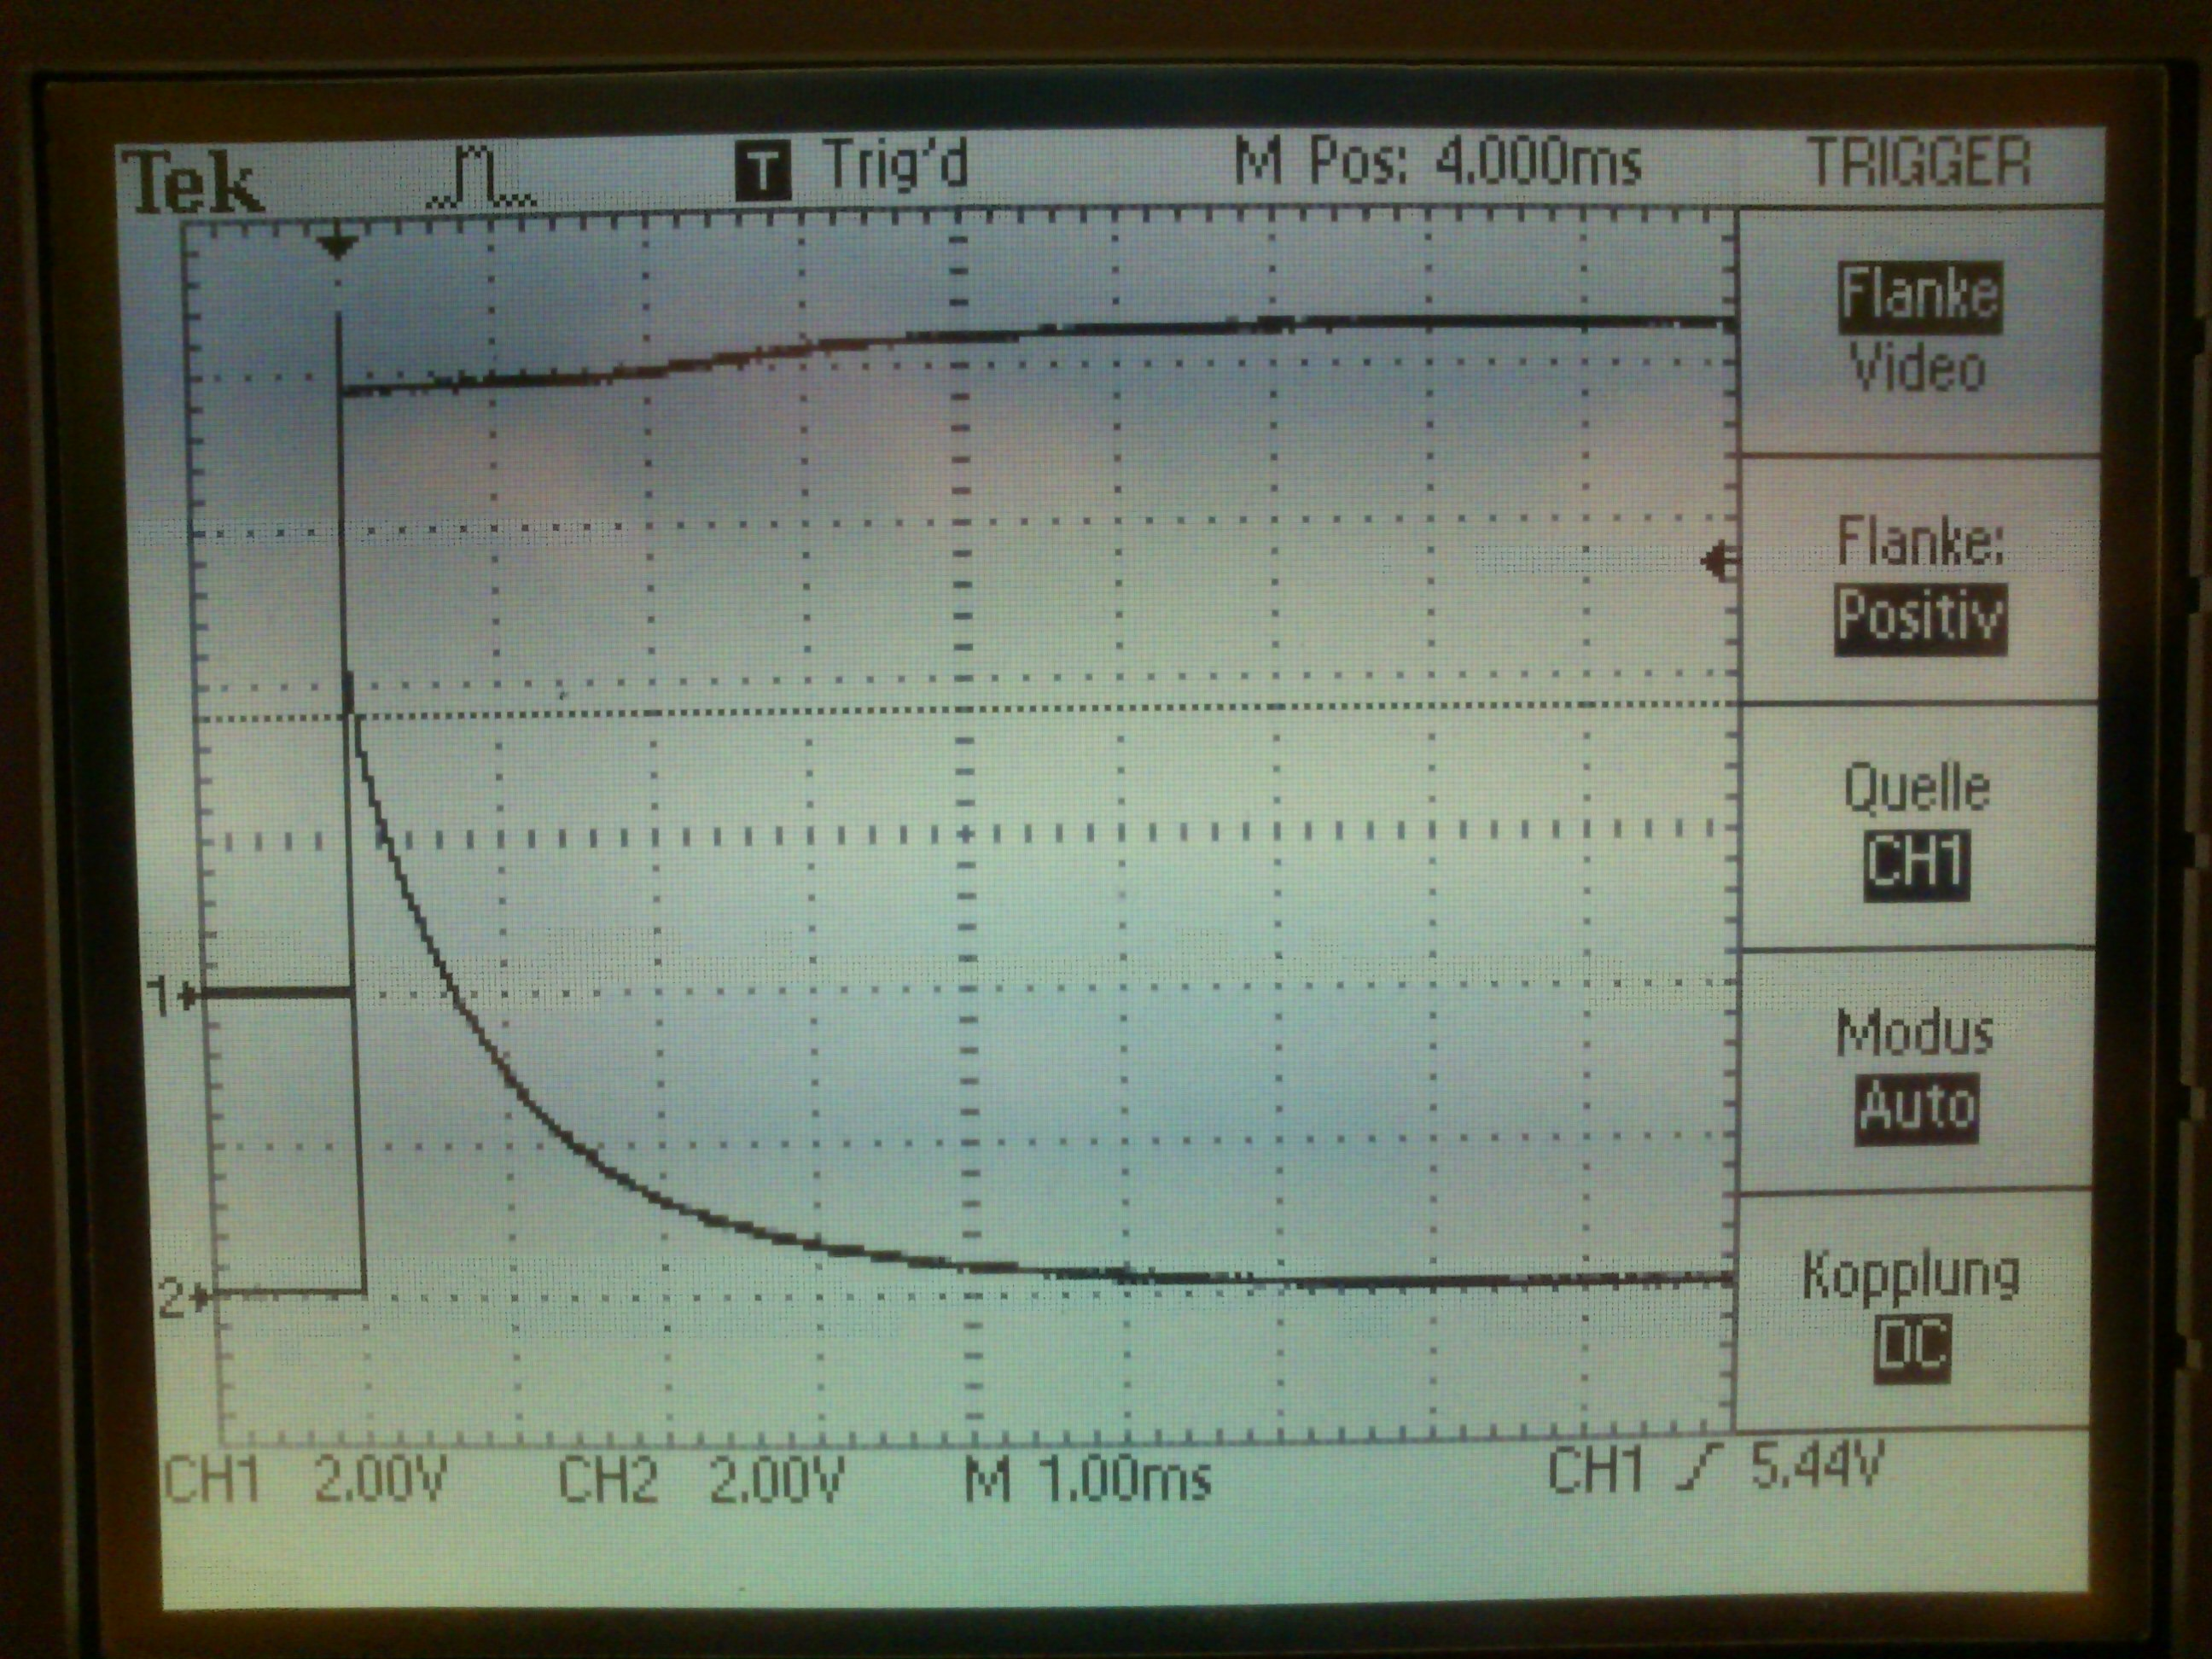
\includegraphics[width=.8\linewidth]{../versuch3/oszibilder/DSC_0287.JPG}
			\caption{Impulsantwort des Hochpasses}
		\end{figure}
	\end{frame}

\section{Untere Grenzfrequenz}

\subsection{Direkte Messung}
\begin{frame}
Hierzu wurde die Frequenz am Generator so lange herunter gedreht, bis die gemessene Spannung am Oszilloskop auf $\sqrt{2}$ mal die Versorgungsspannung abgesunken war:
\begin{figure}[H]
		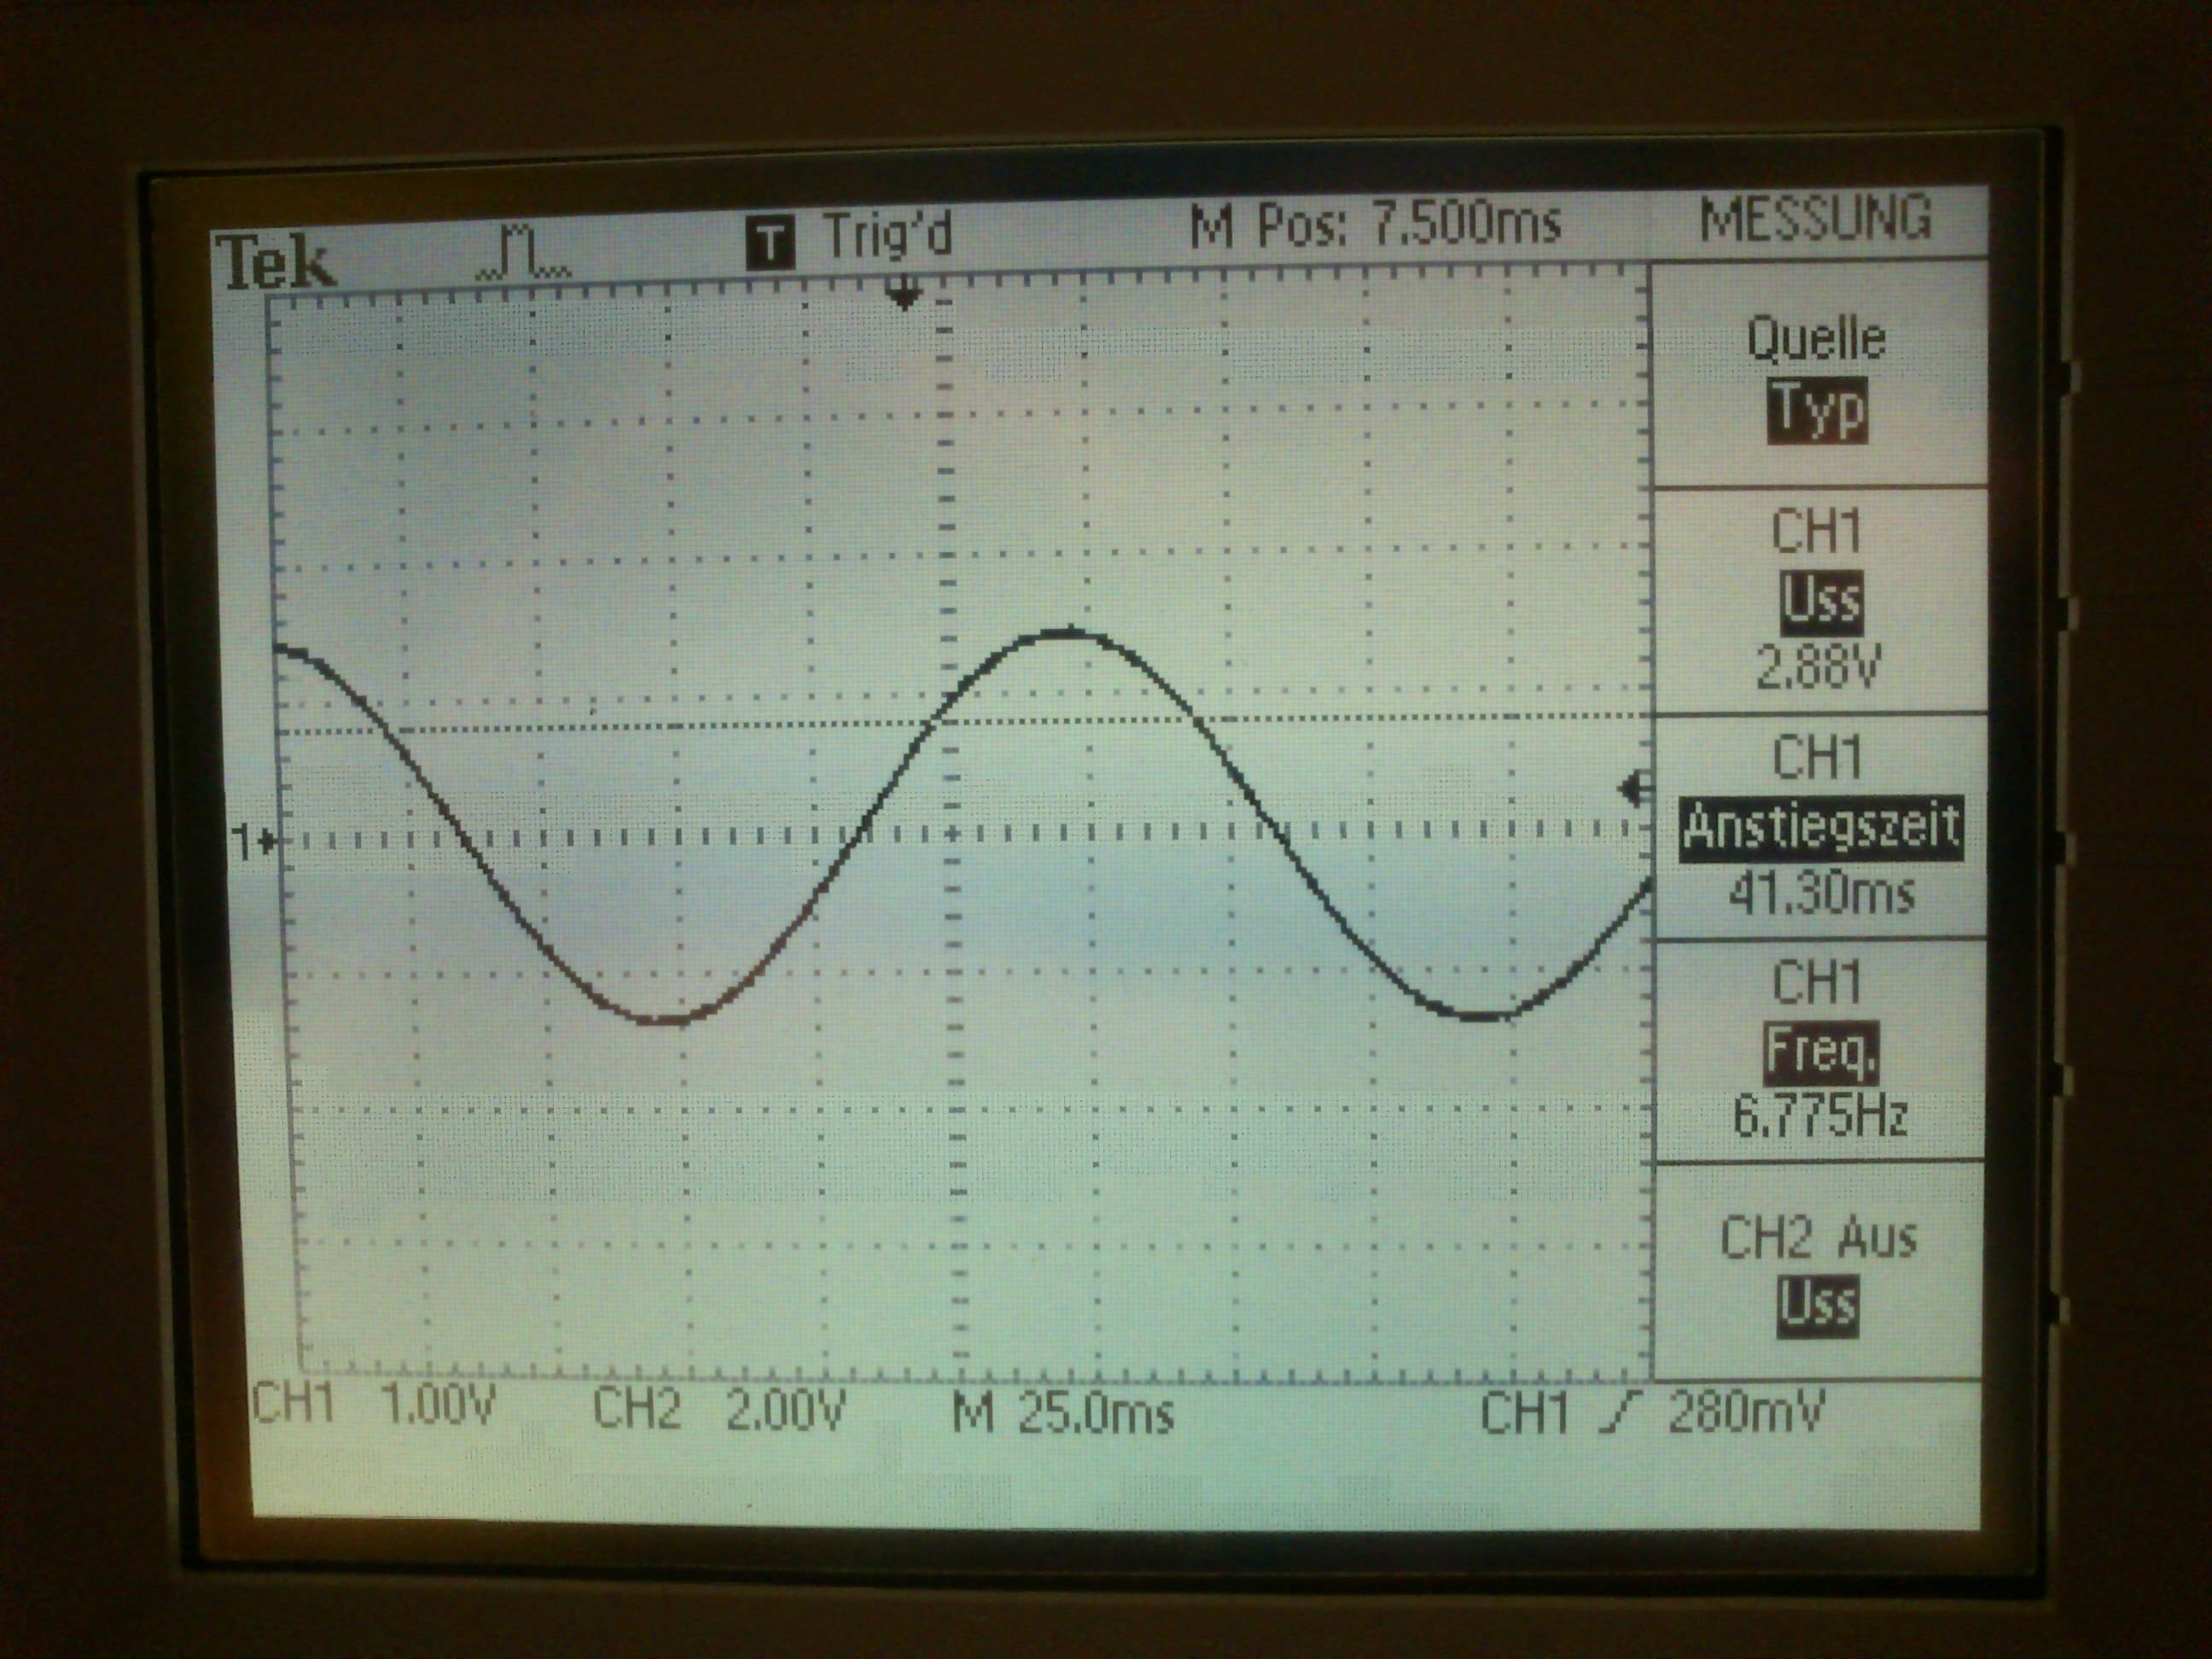
\includegraphics[width=.7\linewidth]{../versuch3/oszibilder/DSC_0295.JPG}
		\caption{Ermittlung der Spannung \ldots}
\end{figure}
\end{frame}

\begin{frame}
\begin{figure}[H]
		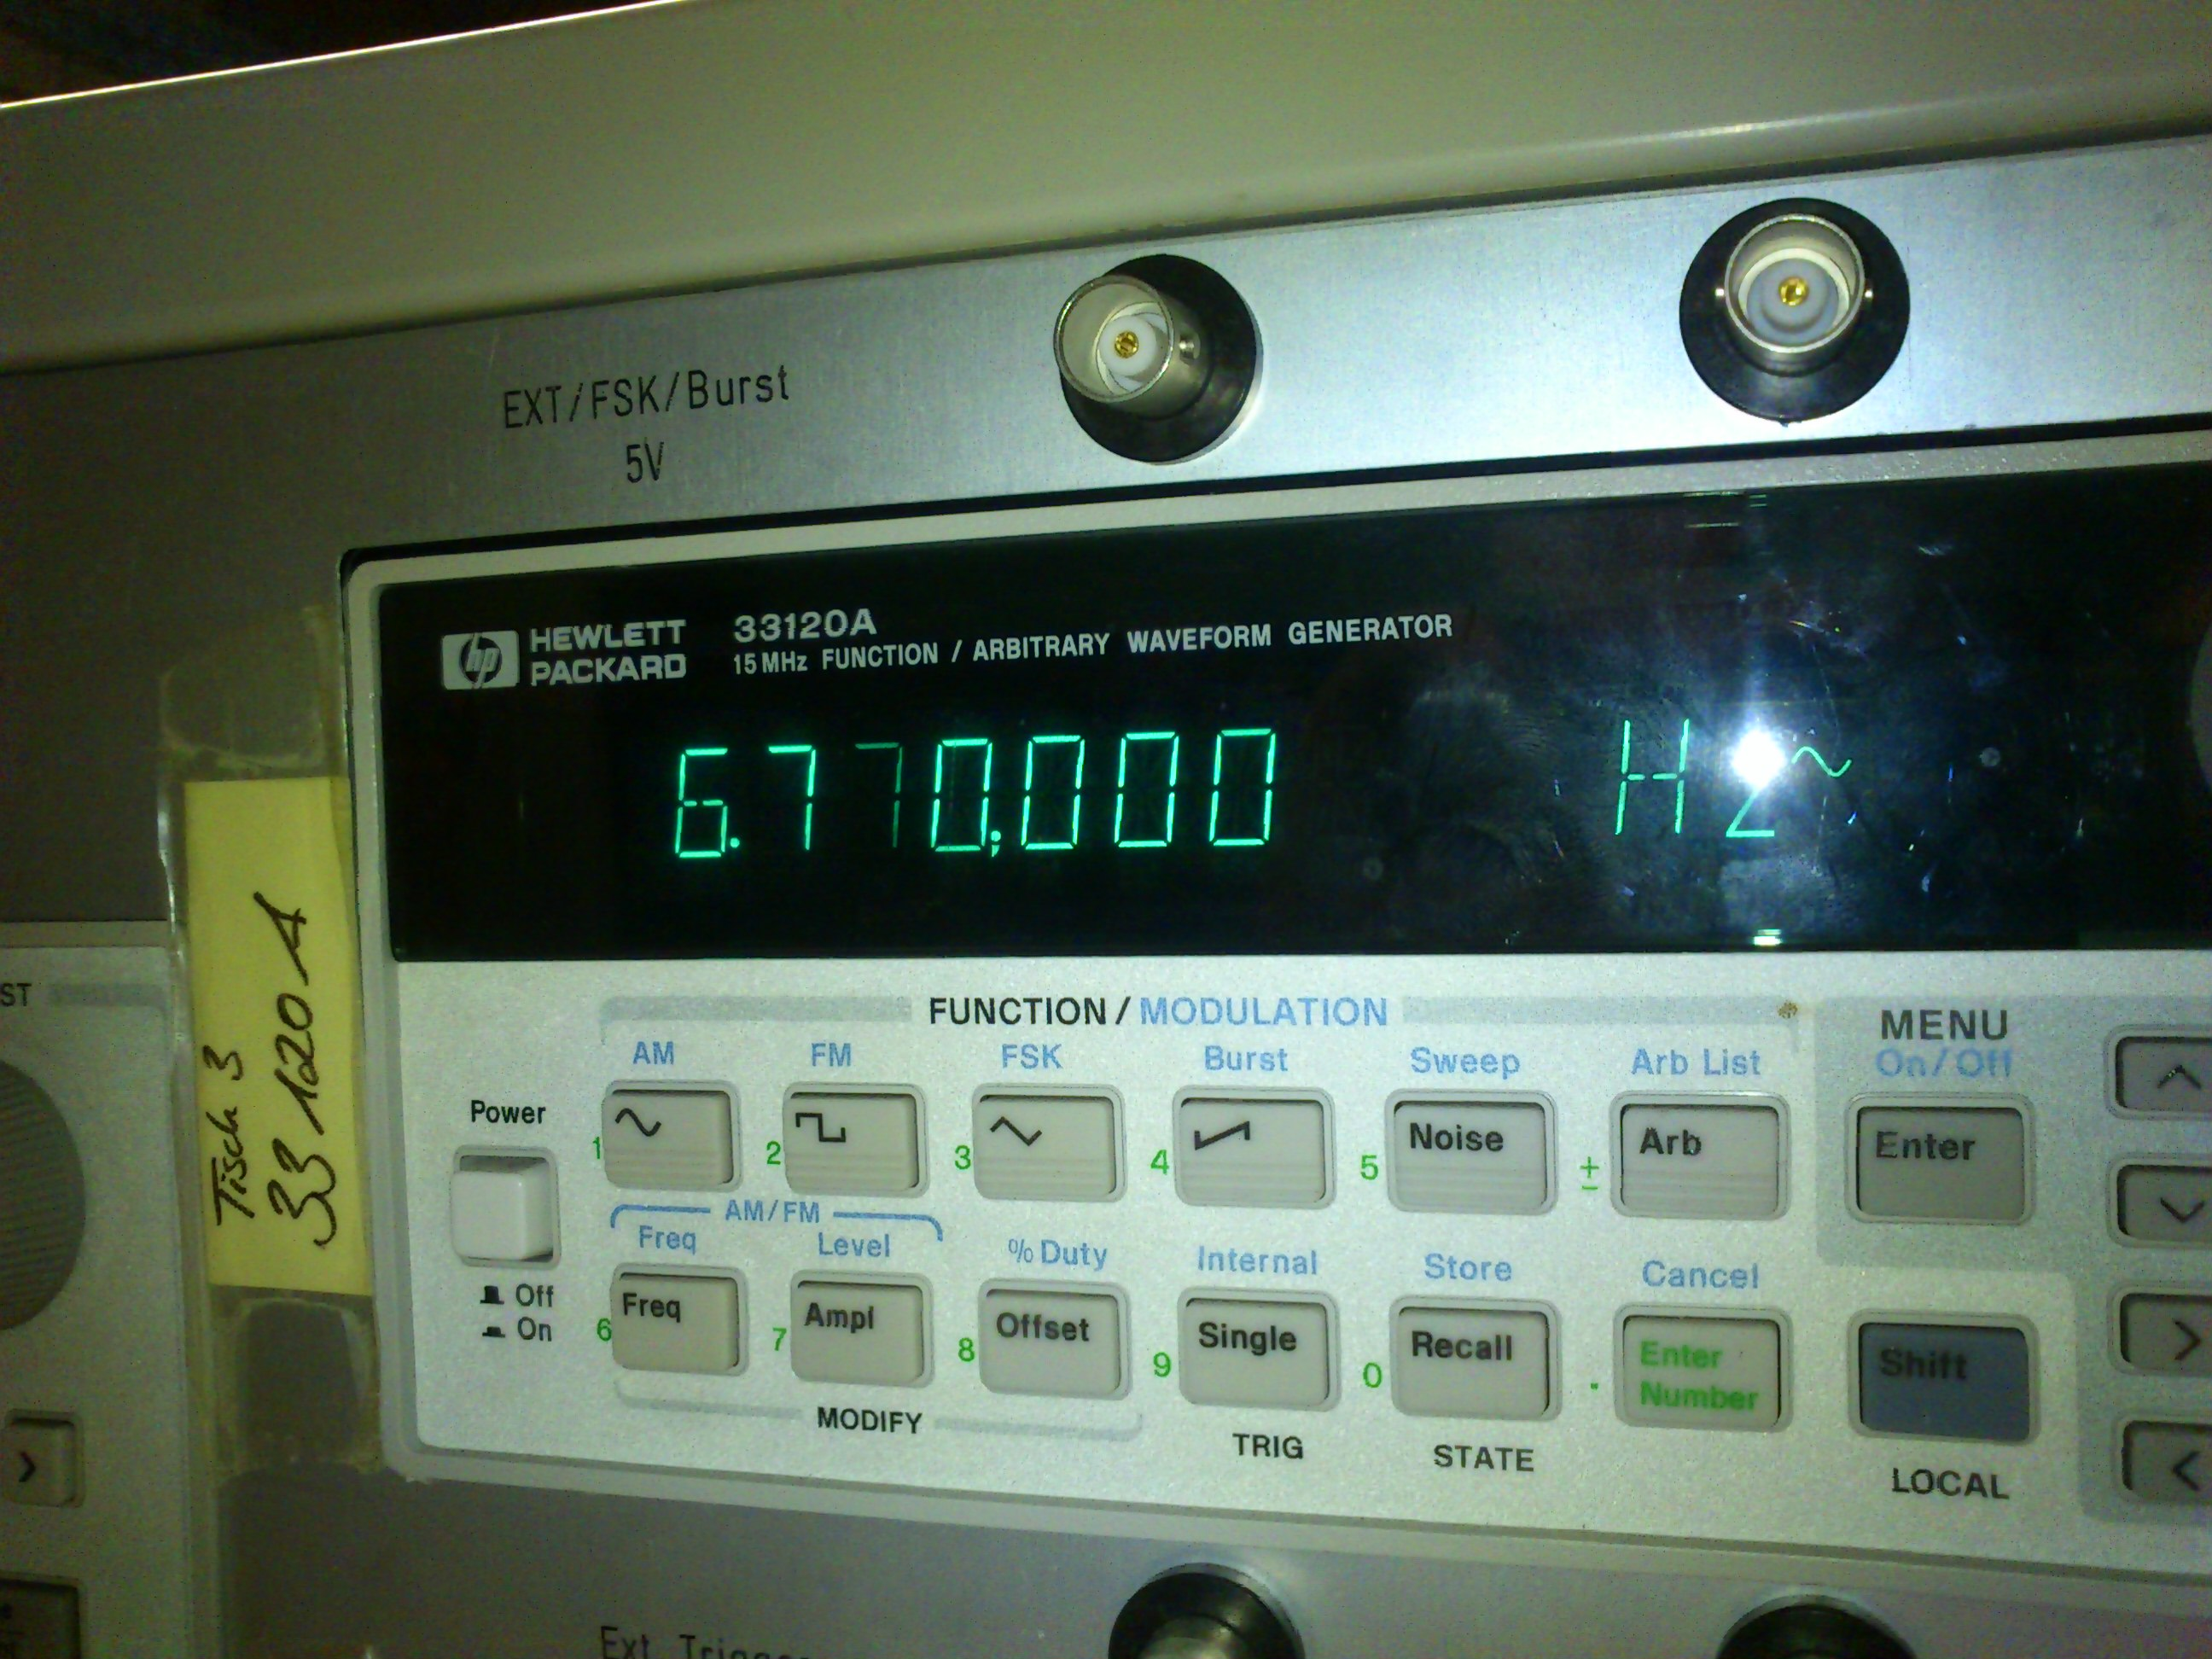
\includegraphics[width=.7\linewidth]{../versuch3/oszibilder/DSC_0294.JPG}
		\caption{\ldots und die Grenzfrequenz}
\end{figure}
Somit ist der untere Grenzwert bei 6.77 Hz.
\end{frame}




\subsection{Dachschräge}
\begin{frame}
	Bei dieser Möglichkeit wird die Dachschräge einer Rechteckspannung für die Messung der unteren Grenzfrequenz herangezogen:
	\begin{figure}[H]
		\centering
		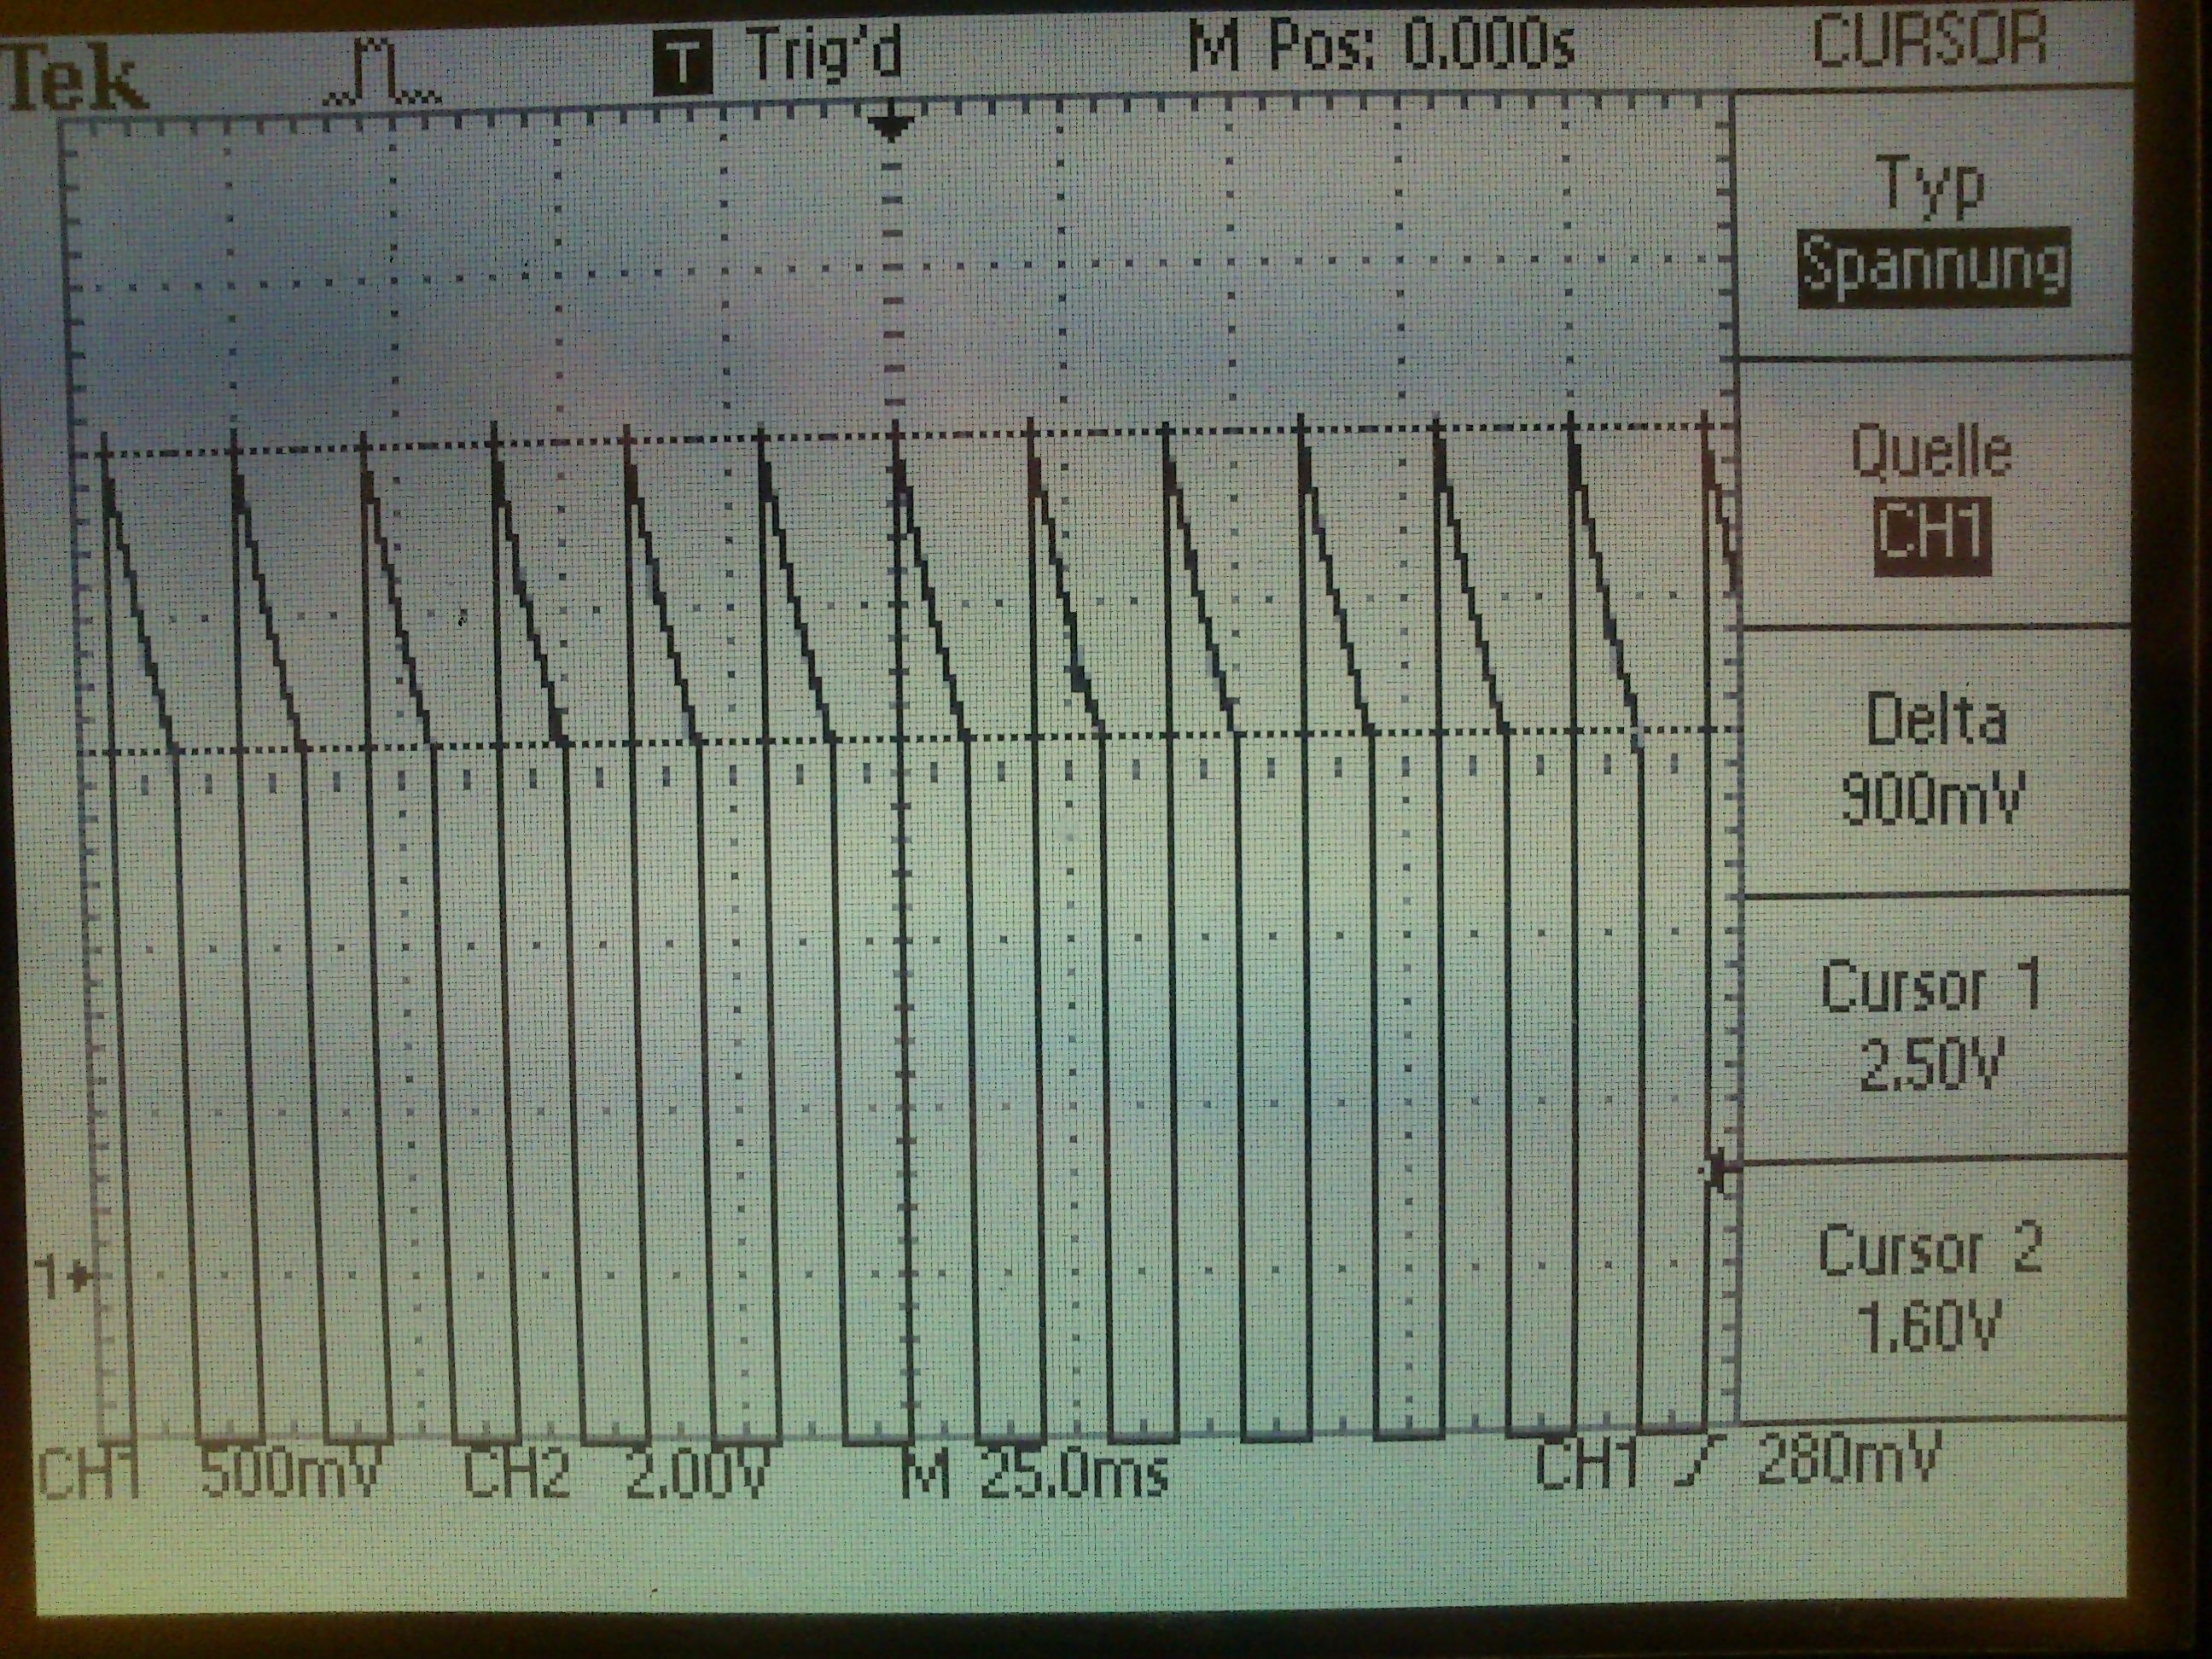
\includegraphics[width=.7\linewidth]{../versuch3/oszibilder/DSC_0300.JPG}
		\caption{Dachschrägenmessung an einer 50Hz-Rechteckspannung: Delta U}
	\end{figure}
\end{frame}
\begin{frame}
	\begin{figure}[H]
		\centering
		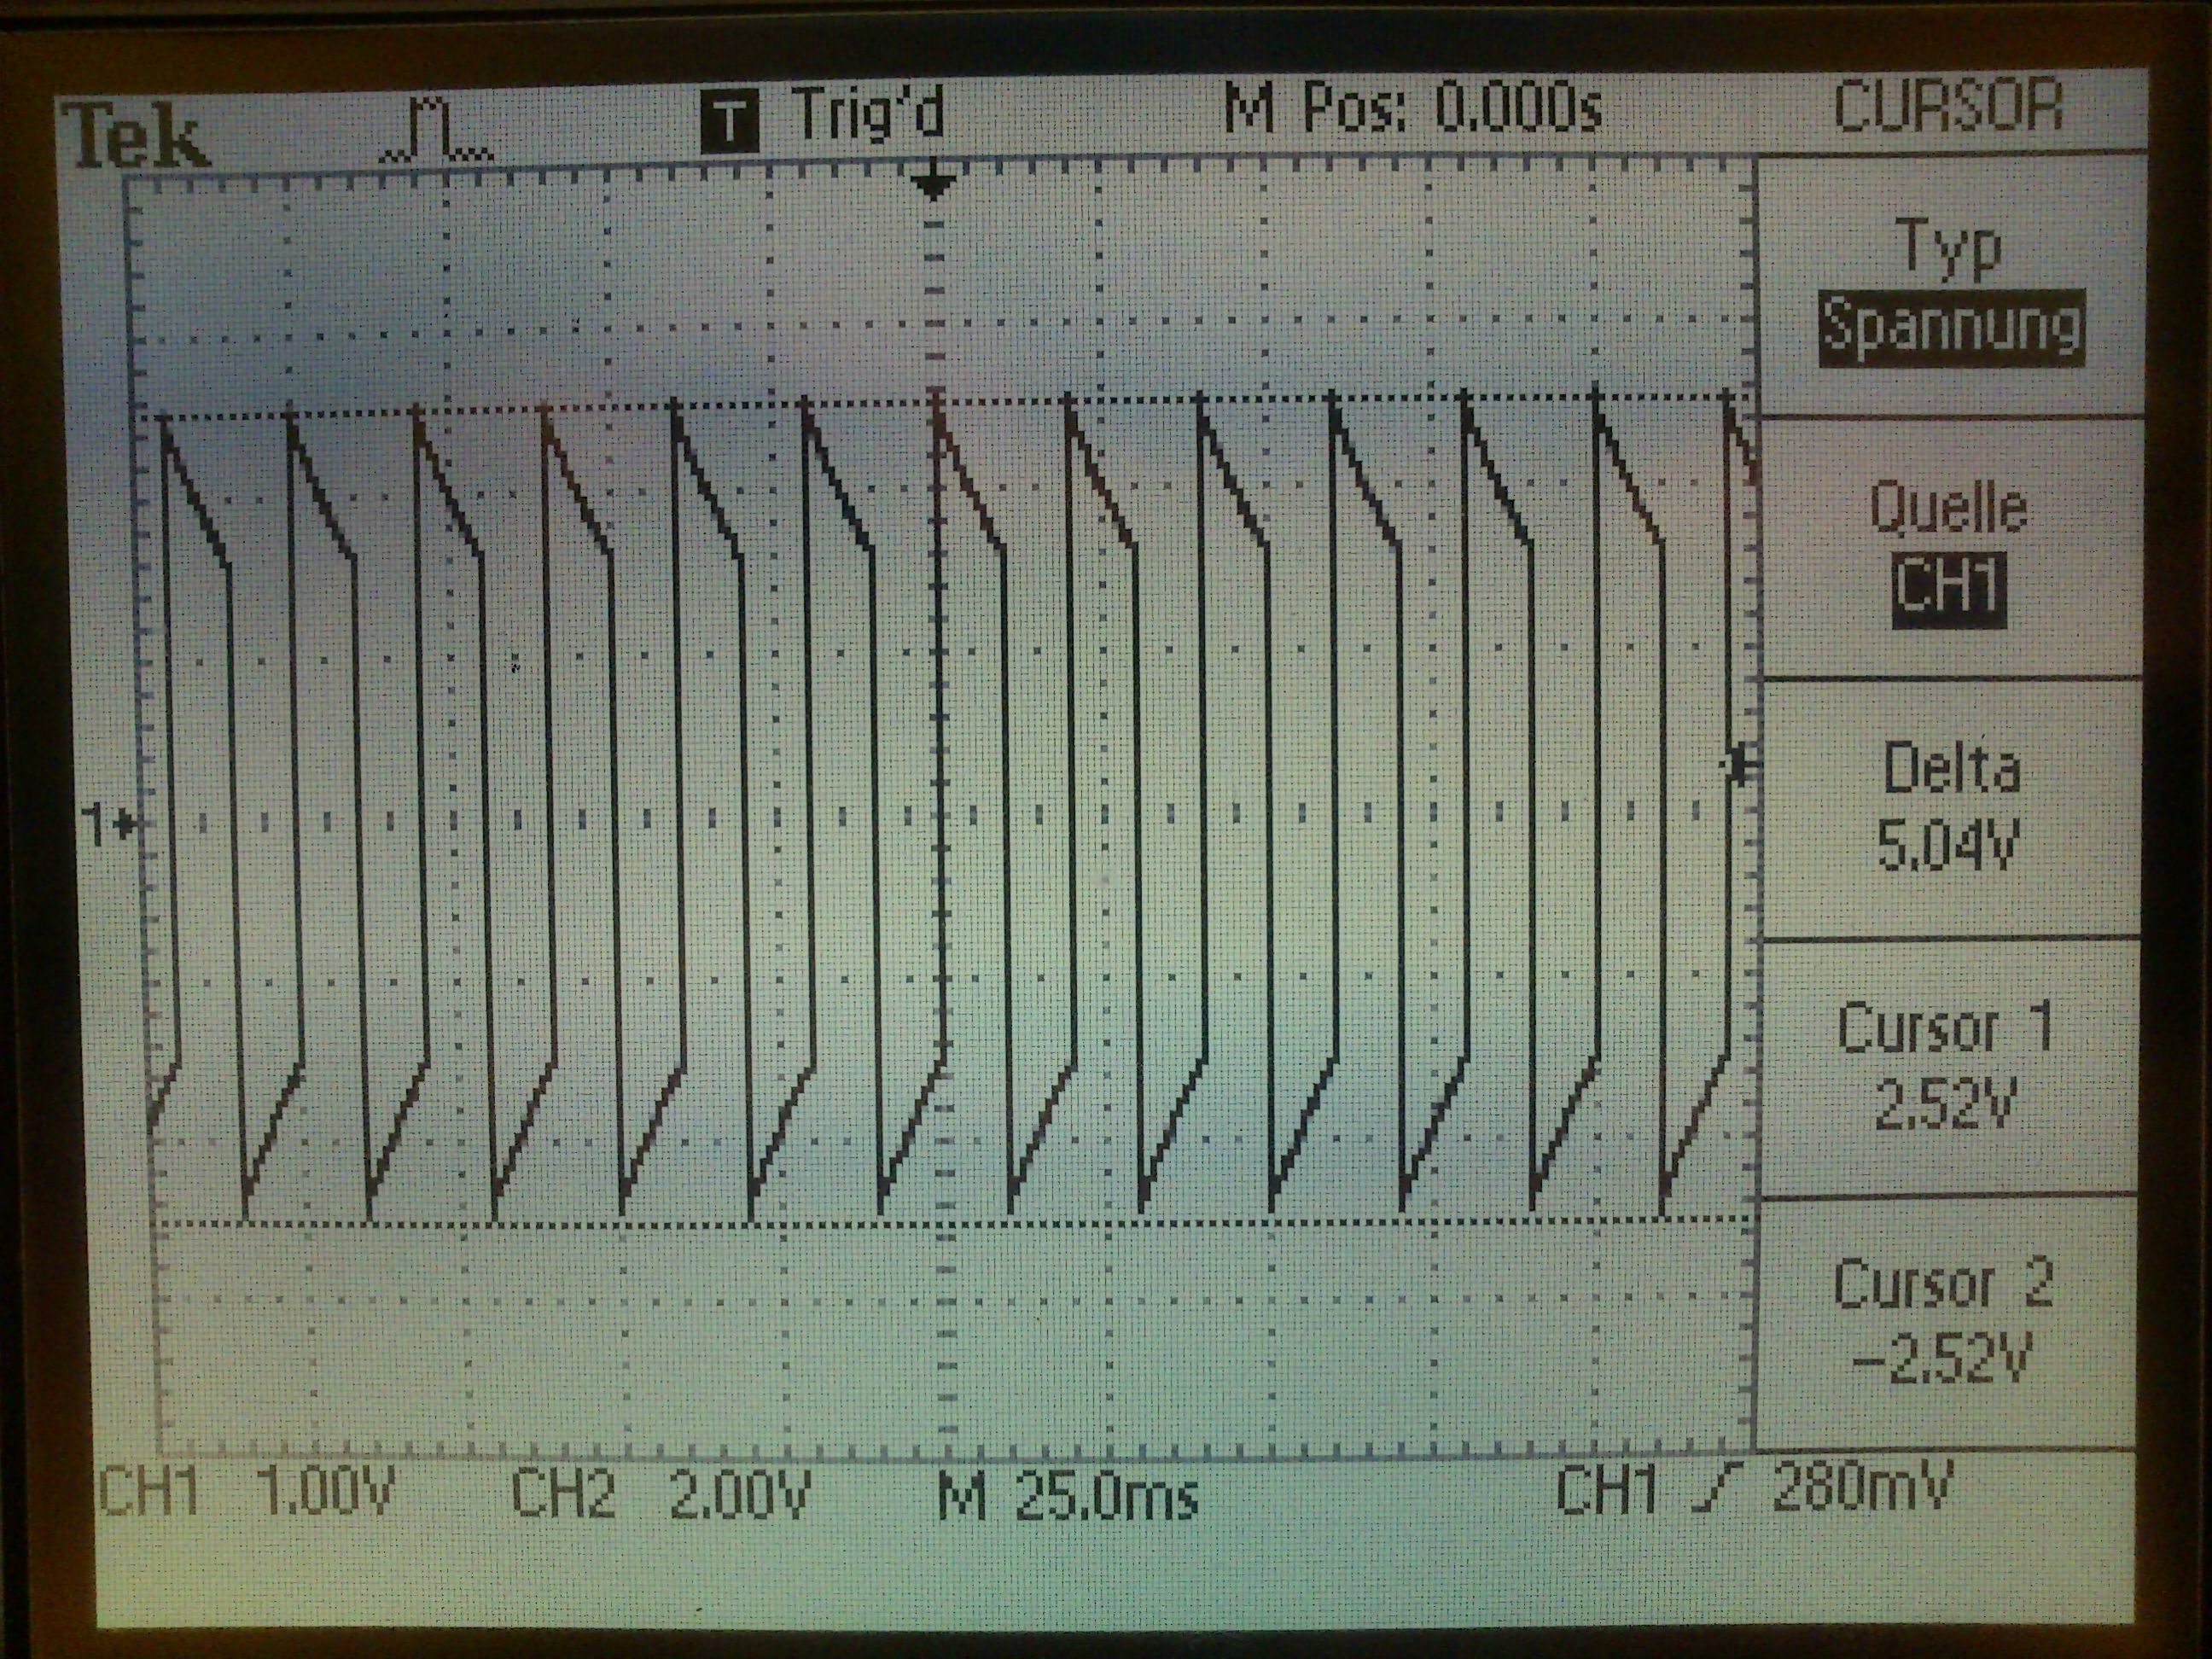
\includegraphics[width=.7\linewidth]{../versuch3/oszibilder/DSC_0304.JPG}
		\caption{Dachschrägenmessung an einer 50Hz-Rechteckspannung: U\textsubscript{ss}}
	\end{figure}
\end{frame}
\begin{frame}
	Damit lässt sich die untere Grenzfrequenz wie folgt berechnen:\\
	$ D = 2 * \frac{∆U}{U_{ss}}=2*\frac{0.9V}{5.04V};\; f=50Hz $ \\
	$ \Rightarrow f_{gu}=\frac{f}{\pi} * ln \frac{1}{1 – D} = \frac{50Hz}{\pi}*ln\frac{1}{1-D} = 7.032 Hz $\\
\end{frame}


\section{Obere Grenzfrequenz}
\subsection{Grenzfrequenz}
\begin{frame}
\begin{figure}[H]
	\centering
	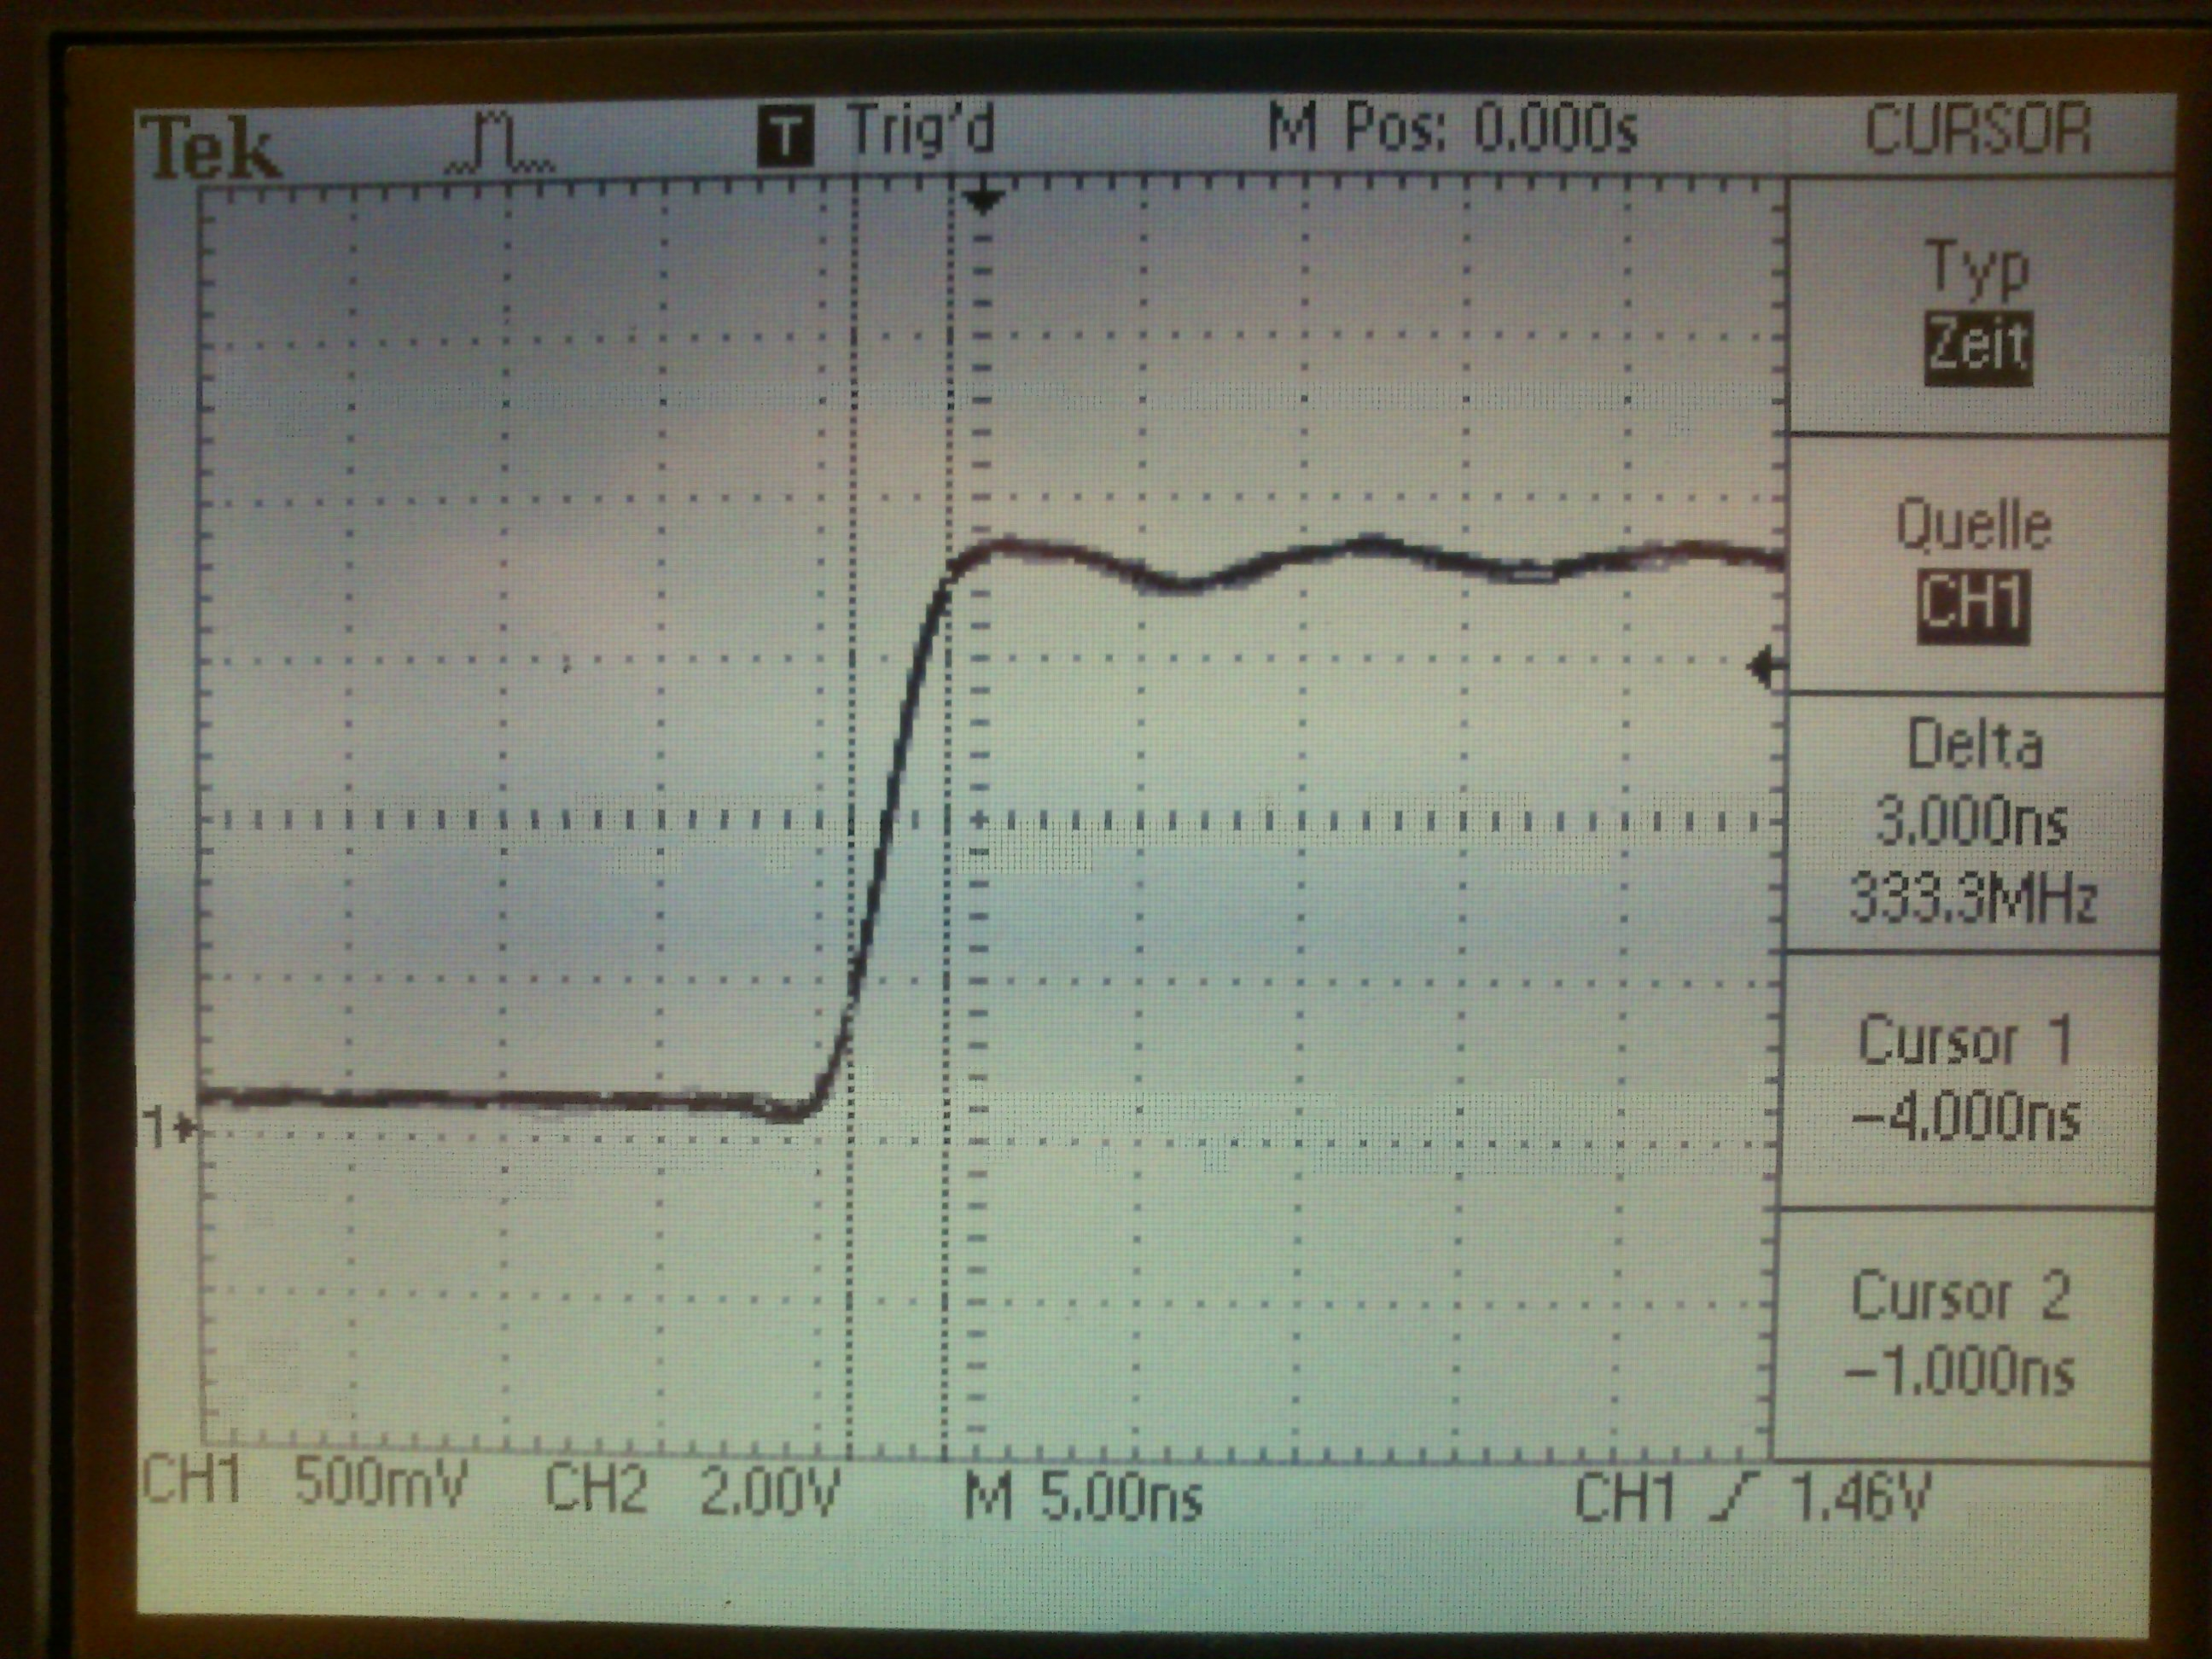
\includegraphics[width=.7\linewidth]{../versuch3/oszibilder/DSC_0313.JPG}
	\caption{Messung der Anstiegszeit T\textsubscript{ges} am Sync-Ausgang}
\end{figure}
\end{frame}
\begin{frame}
Da weiterhin bekannt ist, dass die Eigenanstiegszeit (t\textsubscript{sync}) des Signalgenerators 1,4 ns beträgt, kann man die obere Grenzfrequenz berechnen:\\
$ t_{oszi} = \sqrt{t_ges^2 - t_sync^2} = 2.6533 ns; \; \Rightarrow f_{og} = 0.35/t_oszi = 1.3191*10^8 Hz = 131.91 MHz $
Somit ist die berechnete Frequenz etwa 1,3 mal so groß, wie die Geräteangabe.
\end{frame}

\subsection{Anstiegszeit der Rechteckspannung}
\begin{frame}
\begin{figure}[H]
	\centering
	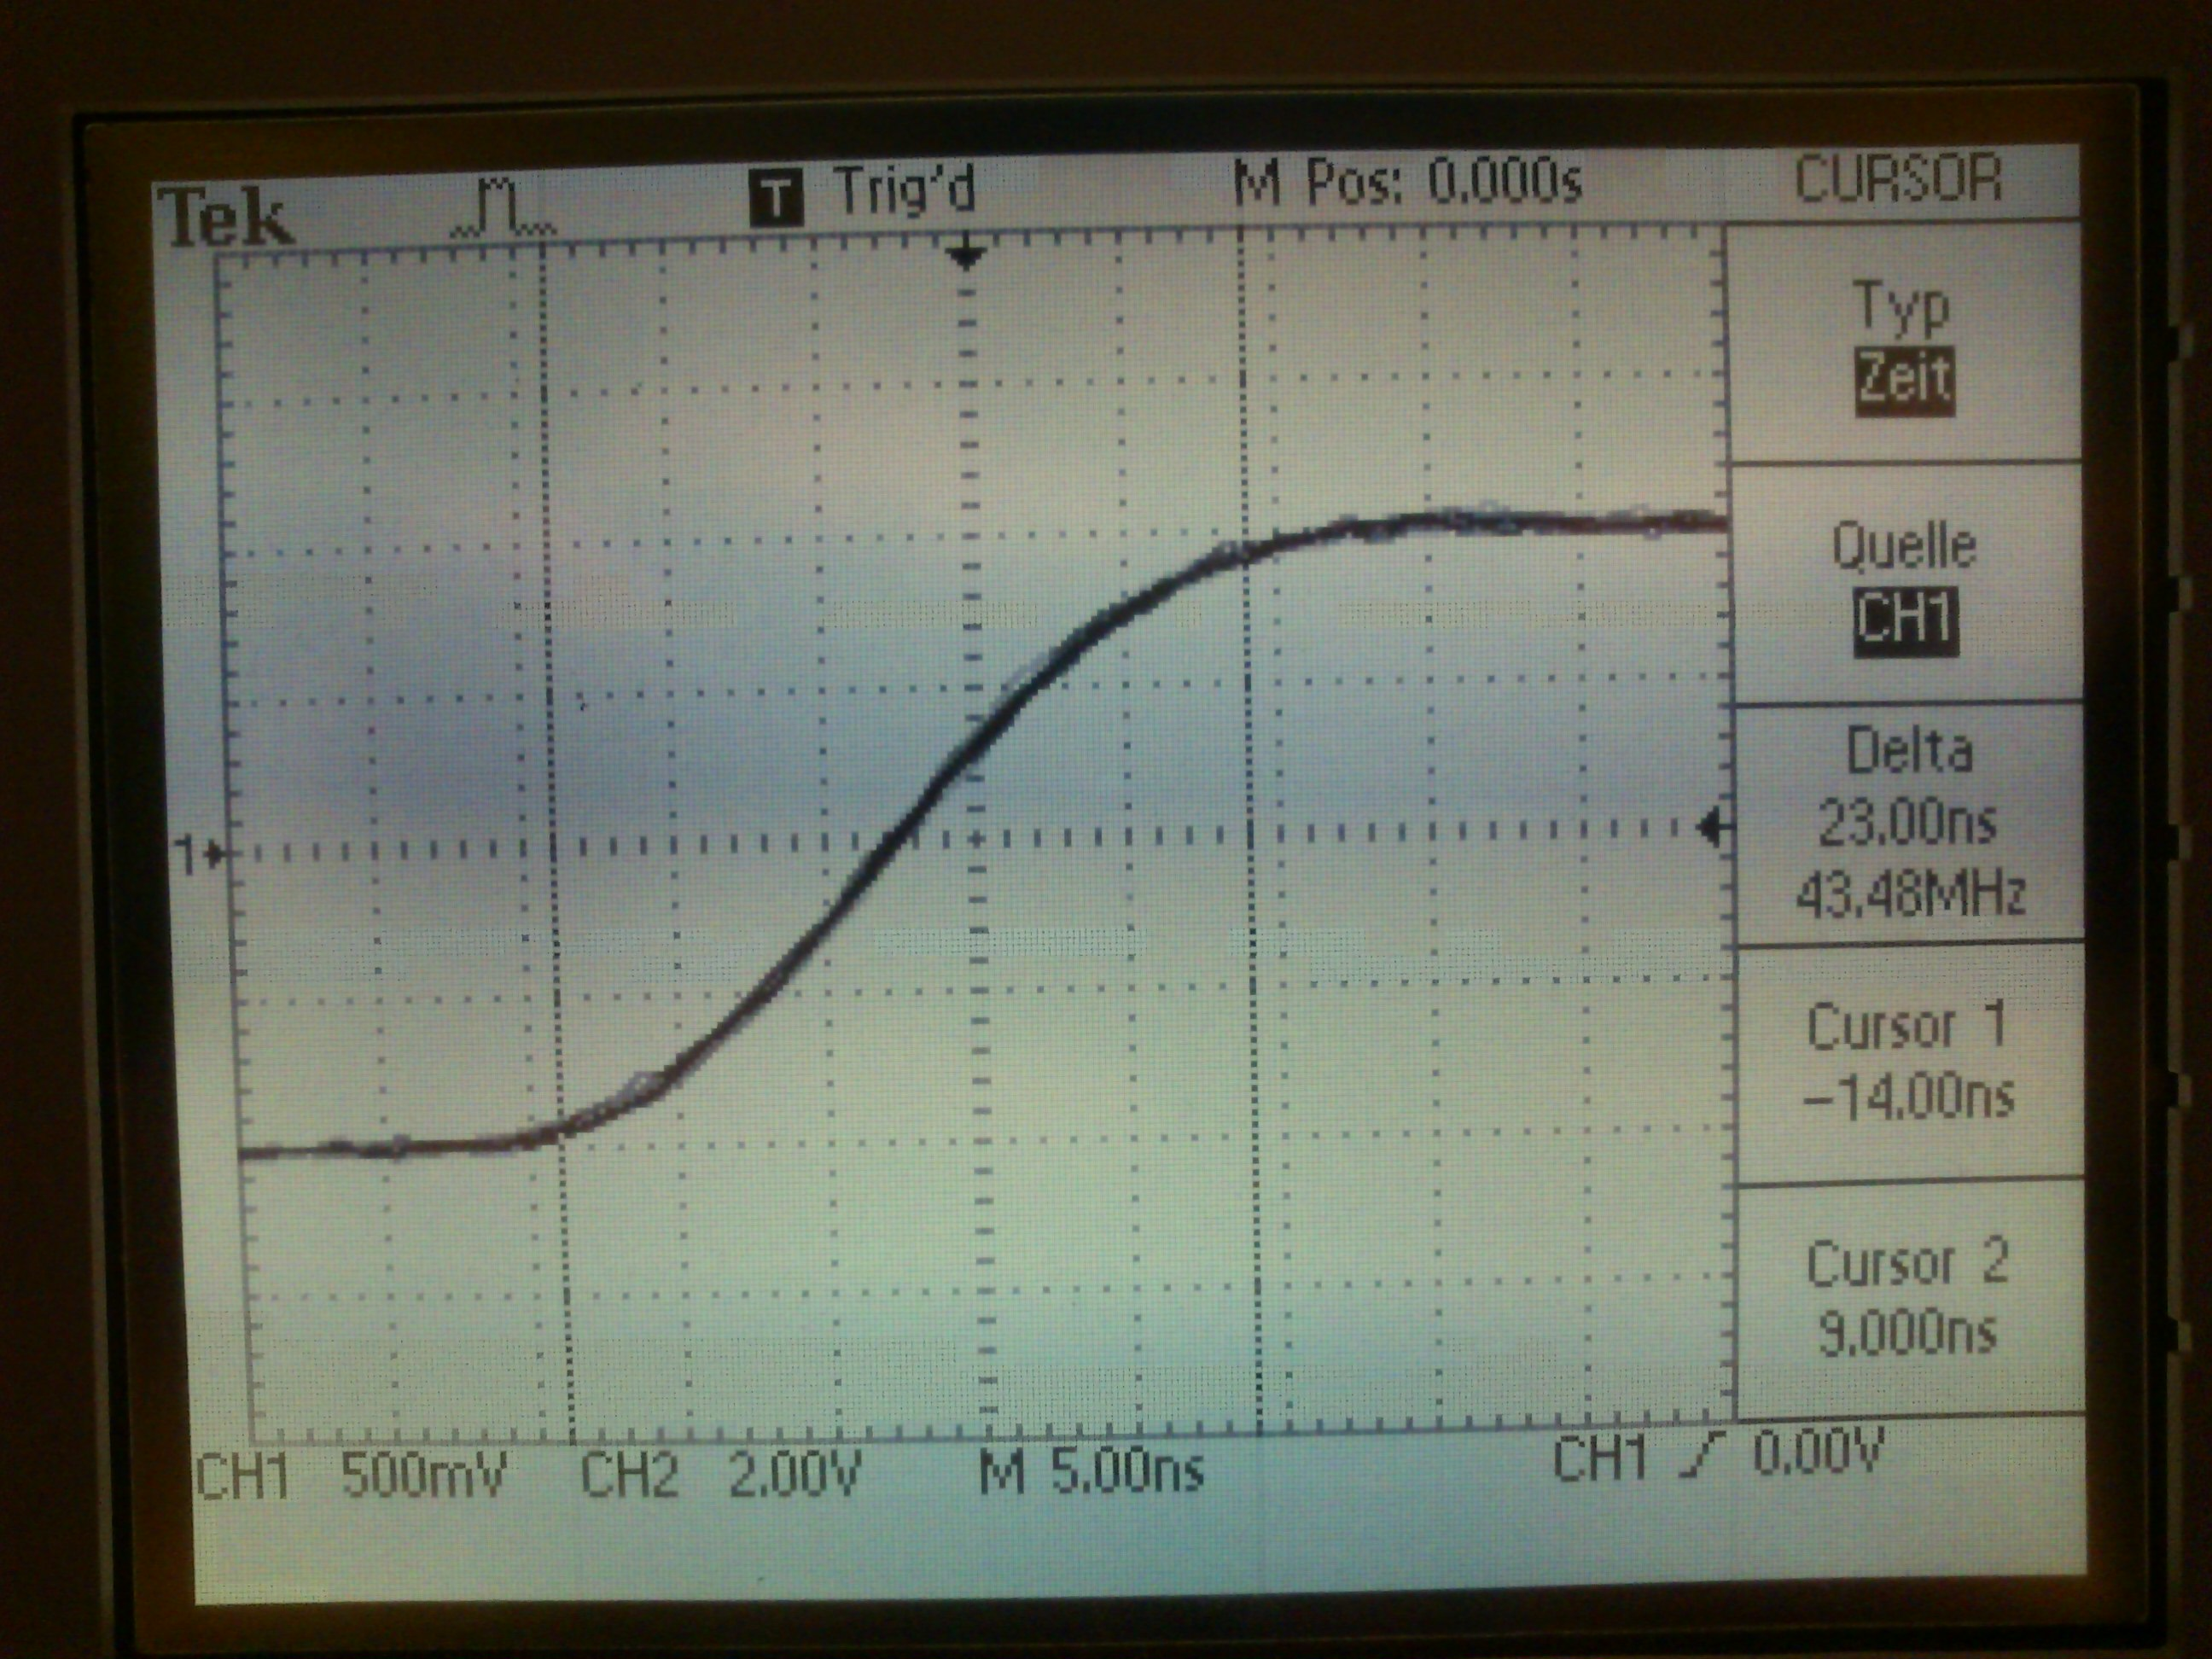
\includegraphics[width=.7\linewidth]{../versuch3/oszibilder/DSC_0318.JPG}
	\caption{Messung der Anstiegszeit normalen Ausgang}
\end{figure}
\end{frame}
\begin{frame}
Damit kann man die Bandbreite des Signals unter Berücksichtigung der Eigenanstiegszeit des Oszilloskops, die zuvor bestimmt wurde, berechnen:
$ t_{sig} = \sqrt{t_{ges}^2 - t_{oszi}^2} = \sqrt{23ns^2 - 2.6533ns^2} = 22.957ns $
\end{frame}

\begin{frame}
	\huge
	ENDE
\end{frame}

\end{document}
%}}}








